\documentclass[11pt]{book}

% Omitting Page Numbers
\pagenumbering{gobble} 

% Packages
\usepackage[a4paper,left=2.5cm,right=2.5cm,top=4cm,bottom=4.9cm]{geometry}
\renewcommand{\baselinestretch}{1.15}
\usepackage{graphicx}
\usepackage{caption}
\usepackage{fontspec}
\usepackage{natbib}
\setcitestyle{square}
\usepackage{afterpage}  % blank pages
\usepackage{multirow}  % table
\usepackage[table, dvipsnames]{xcolor}  % table
\usepackage{xpatch}  % table
\usepackage{tabu}  % table
\usepackage{hhline}  % cell color does not overlap cell line
\usepackage{fancyhdr}  % headers
\usepackage{breakcites}  % references do not go though margins
\usepackage{sectsty}  % change chapter title size
\setcounter{tocdepth}{3}  % four level contents
\setcounter{secnumdepth}{3}  % numbered four level contents
\usepackage{amsfonts}  % math
\usepackage{amsmath}  % math
\usepackage[nottoc,notlof,notlot]{tocbibind}
\usepackage{makecell}
\usepackage{pdflscape}
\usepackage{pdfpages}
\usepackage{subcaption}
\usepackage{float}
\usepackage[pagebackref]{hyperref}  % references

\newcommand{\rectangle}{{  % rectangle
  \ooalign{$\sqsubset\mkern3mu$\cr$\mkern3mu\sqsupset$\cr}
}}

\newcommand\BibTeX{B{\sc ib}\TeX}

% References
\hypersetup{
   colorlinks=true,
   linkcolor=MidnightBlue,
   filecolor=MidnightBlue,
   citecolor=BrickRed,
   urlcolor=MidnightBlue,
   bookmarksopen=true,
   linktocpage=true,
   pdfpagemode=UseOutlines,
   pdfstartpage=1
}

% Blank Page
\newcommand\blankpage{
    \null
    \thispagestyle{empty}
    \addtocounter{page}{-1}
    \newpage}

% Hide Blank Pages Numbers + Headers
\let\origdoublepage\cleardoublepage
\newcommand{\clearemptydoublepage}{%
  \clearpage
  {\pagestyle{empty}\origdoublepage}%
}

% Space between numbers and text
\geometry{footskip=2.45cm}

\begin{document}

\begingroup

\newgeometry{left=3cm, right=3cm, top=1cm, bottom=1.2cm}
\renewcommand{\baselinestretch}{1.9}

\setmainfont{Times New Roman}

\centering{\fontsize{12.2}{14.4}\selectfont UNIVERSIDADE DE LISBOA}\\
\centering{\fontsize{12.2}{14.4}\selectfont FACULDADE DE CIÊNCIAS}\\
%\centering{\fontsize{12.2}{14.4}\selectfont DEPARTAMENTO DE INFORMÁTICA}

\vspace{0.2cm}

\begin{figure}[h]
 \centering
 
\includegraphics[width = 5.5cm,height = 6.5cm]{images/logo.png}
\end{figure}

\centering{\fontsize{12.2}{14.4}\selectfont \textbf{Deep Learning System for Biomedical Relation Extraction \\Combining External Sources of Knowledge}}

\vspace{1cm}

\centering{\fontsize{12.2}{14.4}\selectfont Proposta de Tese}

\vspace{1cm}

\centering{\fontsize{12.2}{14.4}\selectfont \textbf{Doutoramento em Informática}}\\

\vspace{3.5cm}

\centering{\fontsize{12.2}{14.4}\selectfont Diana Francisco de Sousa}

\vspace{1.3cm}


\centering{\fontsize{12.2}{14.4}\selectfont Tese orientada por:}\\
\centering{\fontsize{12.2}{14.4}\selectfont Professor Doutor Francisco José Moreira Couto}

\vspace{4.3cm}

\centering{\fontsize{12.2}{14.4}\selectfont 2020}

\setmainfont{Times New Roman}

\centering{\fontsize{12.2}{14.4}\selectfont UNIVERSIDADE DE LISBOA}\\
\centering{\fontsize{12.2}{14.4}\selectfont FACULDADE DE CIÊNCIAS}\\
%\centering{\fontsize{12.2}{14.4}\selectfont DEPARTAMENTO DE INFORMÁTICA}

\vspace{0.2cm}

\begin{figure}[h]
 \centering
 
\includegraphics[width = 5.5cm,height = 6.5cm]{images/logo.png}
\end{figure}

\centering{\fontsize{12.2}{14.4}\selectfont \textbf{Deep Learning System for Biomedical Relation Extraction \\Combining External Sources of Knowledge}}

\vspace{2cm}

%\centering{\fontsize{12.2}{14.4}\selectfont Proposta de Tese}


\centering{\fontsize{12.2}{14.4}\selectfont \textbf{Doutoramento em Informática}}\\

\vspace{2cm}

\centering{\fontsize{12.2}{14.4}\selectfont Diana Francisco de Sousa}

\vspace{1.3cm}


\centering{\fontsize{12.2}{14.4}\selectfont Tese orientada por:}\\
\centering{\fontsize{12.2}{14.4}\selectfont Professor Doutor Francisco José Moreira Couto}

\vspace{2cm}

\centering{\fontsize{12.2}{14.4}\selectfont This work was supported by FCT through funding of DeST: Deep Semantic Tagger project, ref. PTDC/CCI-BIO/28685/2017 (http://dest.rd.ciencias.ulisboa.pt/), LASIGE Research Unit, ref. UIDB/00408/2020, and PhD Scholarship, ref. SFRH/BD/145221/2019.
}

\vspace{1.3cm}

%\vspace{4.3cm}

\centering{\fontsize{12.2}{14.4}\selectfont 2020}


\afterpage{\blankpage}

\endgroup

% Preamble for Thesis
\setmainfont{Times New Roman}
\newgeometry{left=2.5cm,right=2.5cm,top=2.5cm,bottom=4.9cm}
\renewcommand{\baselinestretch}{1.15}
\pagenumbering{Roman}
\pagestyle{plain}
\let\cleardoublepage\clearemptydoublepage  % hide blank pages numbers + headers

%\chapter*{\begin{center}Acknowledgements\end{center}}

\noindent{Firstly, I would like to offer my special thanks to my teacher and supervisor, Professor Francisco Couto, for his guidance and support throughout this project. I also want to thank André Lamúrias, for his suggestions and corrections that were extremely important for the development, and conclusion of this dissertation. To my day-to-day LASIGE colleagues (Márcia, Telma, Joana, Sofia, Alexandra, Soraia, Miguel, Vinícius, Nuno, Adriano, Fernando, Rita, Margarida, Teresa, and Sofia), for coffee, lunch, and for all the great team spirit and working environment. To my friend Beatriz Lopes, for being present at every step of the way, understanding every struggle and every success. To all my other dear friends (Sofia, Clara, Íris, and Inês) with whom I can always count for great conversations and support, wherever they are in the world. To my parents that allowed me to have all these amazing opportunities, and believed in me always. To my sister for always having my back, and making me proud of her every day. Finally, I would like to thank Rafael Ramos for unconditional love and support.}

%\chapter*{\begin{center}Resumo\end{center}}

\noindent{As relações entre fenótipos humanos e genes são fundamentais para entender completamente a origem de algumas abnormalidades fenotípicas e as suas doenças associadas. A literatura biomédica é a fonte mais abrangente dessas relações. Diversas ferramentas de extração de relações têm sido propostas para identificar relações entre conceitos em texto muito heterogéneo ou não estruturado, utilizando algoritmos de supervisão distante e aprendizagem profunda. Porém, a maioria dessas ferramentas requer um \textit{corpus} anotado e não há nenhum \textit{corpus} disponível anotado com relações entre fenótipos humanos e genes.} 

Este trabalho apresenta o \textit{corpus} \textit{Phenotype-Gene Relations} (PGR), um \textit{corpus} padrão-prata de anotações de fenótipos humanos e genes e as suas relações (gerado de forma automática) e dois módulos de extração de relações usando um algoritmo de \textit{distantly supervised multi-instance learning} e um algoritmo de aprendizagem profunda com ontologias biomédicas. 
O \textit{corpus} PGR consiste em 1712 resumos de artigos, 5676 anotações de fenótipos humanos, 13835 anotações de genes e 4283 relações. Os resultados do \textit{corpus} foram parcialmente avaliados por oito curadores, todos investigadores nas áreas de Biologia e Bioquímica, obtendo uma precisão de 87,01\%, com um valor de concordância inter-curadores de 87,58\%. 
As abordagens de supervisão distante (ou supervisão fraca) combinam um \textit{corpus} não anotado com uma base de dados para identificar e extrair entidades do texto, reduzindo a quantidade de esforço necessário para realizar anotações manuais. A \textit{distantly supervised multi-instance learning} aproveita a supervisão distante e um \textit{sparse multi-instance learning algorithm} para treinar um classificador de extração de relações, usando uma base de dados padrão-ouro de relações entre fenótipos humanos e genes. 
As ferramentas de aprendizagem profunda de extração de relações, para tarefas de prospeção de textos biomédicos, raramente tiram proveito dos recursos específicos existentes para cada domínio, como as ontologias biomédicas. As ontologias biomédicas desempenham um papel fundamental, fornecendo informações semânticas e de ancestralidade sobre uma entidade. Este trabalho utilizou a \textit{Human Phenotype Ontology} e a \textit{Gene Ontology}, para representar cada par candidato como a sequência de relações entre os seus ancestrais para cada ontologia. 
O \textit{corpus} de teste PGR foi aplicado aos módulos de extração de relações desenvolvidos, obtendo resultados promissores, nomeadamente 55,00\% (módulo de aprendizagem profunda) e 73,48\% (módulo de \textit{distantly supervised multi-instance learning}) na medida-F. Este \textit{corpus} de teste também foi aplicado ao BioBERT, um modelo de representação de linguagem biomédica pré-treinada para prospeção de texto biomédico, obtendo 67,16\% em medida-F.

\vspace{0.5cm}

\textbf{Palavras Chave:} Literatura Biomédica, Extração de Relações, \textit{Corpus} Padrão-Prata, Supervisão Distante, Aprendizagem Profunda. 


\chapter*{\begin{center}Abstract\end{center}}

\noindent{Human phenotype-gene relations are fundamental to fully understand the origin of some phenotypic abnormalities and their associated diseases. Biomedical literature is the most comprehensive source of these relations. Several relation extraction tools have been proposed to identify relations between concepts in highly heterogeneous or unstructured text, namely using distant supervision and deep learning algorithms. However, most of these tools require an annotated corpus, and there is no corpus available annotated with human phenotype-gene relations.}

This work presents the Phenotype-Gene Relations (PGR) corpus, a silver standard corpus of human phenotype and gene annotations and their relations (generated in a fully automated manner), and two relation extraction modules using a distantly supervised multi-instance learning algorithm, and an ontology-based deep learning algorithm.
The PGR corpus consists of 1712 abstracts, 5676 human phenotype annotations, 13835 gene annotations, and 4283 relations. The corpus results were partially evaluated by eight curators, all working in the fields of Biology and Biochemistry, obtaining a precision of 87.01\%, with an inter-curator agreement score of 87.58\%.
Distant supervision (or weak supervision) approaches combine an unlabeled corpus with a knowledge base to identify and extract entities from text, reducing the amount of manual effort necessary. Distantly supervised multi-instance learning takes advantage of distant supervision and a sparse multi-instance learning algorithm to train a relation extraction classifier, using a gold standard knowledge base of human phenotype-gene relations.  
Deep learning relation extraction tools, for biomedical text mining tasks, rarely take advantage of existing domain-specific resources, such as biomedical ontologies. Biomedical ontologies play a fundamental role by providing semantic and ancestry information about an entity. This work used the Human Phenotype Ontology and the Gene Ontology, to represent each candidate pair as the sequence of relations between its ancestors for each ontology.
The PGR test-set was applied to the developed relation extraction modules, obtaining promising results, namely 55.00\% (deep learning module), and 73.48\% (distantly supervised multi-instance learning module) in F-measure. This test-set was also applied to BioBERT, a pre-trained biomedical language representation model for biomedical text mining, obtaining 67.16\% in F-measure.

\vspace{0.5cm}

\textbf{Keywords:} Biomedical Literature, Relation Extraction, Silver Standard Corpus, Distant Supervision, Deep Learning. 



%\chapter*{\begin{center}Resumo Alargado\end{center}}

\noindent{A literatura biomédica é o principal meio que os investigadores utilizam para partilhar as suas descobertas, maioritariamente na forma de artigos, patentes e outros tipos de relatórios escritos. Um investigador interessado num tópico específico precisa de estar atualizado em relação aos trabalhos desenvolvidos sobre esse tópico. No entanto, o volume de informação textual disponível supera amplamente a capacidade de análise de um investigador, mesmo restringindo a um domínio específico. Não só isso, mas a informação textual disponível é geralmente apresentada num formato não estruturado ou altamente heterogéneo. Assim, a recuperação de informação relevante exige não só uma quantidade considerável de esforço manual, mas também é uma tarefa que consome demasiado tempo.}

Os artigos científicos são a principal fonte de conhecimento para entidades biomédicas e as suas relações. Essas entidades incluem fenótipos humanos, genes, proteínas, substâncias químicas, doenças e outras entidades biomédicas inseridas em domínios específicos. Uma fonte abrangente de artigos sobre este tópico é a plataforma PubMed, que combina mais de 29 milhões de citações, fornecendo acesso aos seus metadados. O processamento desse volume de informação só é viável através de soluções de prospeção de texto. 

Os métodos automáticos de Extração de Informação (EI) visam obter informações úteis de grandes conjuntos de dados. As soluções de prospeção de texto usam métodos de EI para processar documentos de texto. Os sistemas de prospeção de texto geralmente incluem tarefas de \textit{Named-Entity Recognition} (NER), \textit{Named-Entity Linking} (NEL) e Extração de Relações (ER). O NER consiste em reconhecer entidades mencionadas no texto, identificando o seu primeiro e último carácter. O NEL consiste em mapear as entidades reconhecidas a entradas numa determinada base de dados. A ER consiste em identificar relações entre as entidades mencionadas num determinado documento. Algumas das relações biomédicas comummente extraídas são as interações proteína-proteína, interações fármaco-fármaco e relações gene-doença.

A ER pode ser executada por diferentes métodos, a saber, por ordem de complexidade: coocorrência, baseados em padrões (criados manual e automaticamente), baseados em regras (criados manualmente e automaticamente) e aprendizagem automática (\textit{feature-based}, \textit{kernel-based}, \textit{multi-instance} (MIL) e \textit{recurrent neural networks} (RNN)). O método de \textit{distantly supervised multi-instance learning} utiliza uma base de dados de relações padrão-ouro do domínio de interesse (supervisão distante) combinada com um \textit{sparse multi-instance learning algorithm} (sMIL) para executar a ER. A supervisão distante pressupõe que qualquer frase que mencione um par de entidades correspondente a uma entrada na base de dados provavelmente descreverá uma relação entre essas entidades. Essas relações candidatas podem ser usadas para treinar um classificador usando o algoritmo sMIL. Mais recentemente, técnicas de aprendizagem profunda, como a RNN, provaram obter excelentes resultados em várias tarefas de Processamento de Linguagem Natural (PNL), entre elas a ER. O sucesso da aprendizagem profunda para a PNL biomédica deve-se em parte ao desenvolvimento de modelos de vectores de palavras como o Word2Vec e, mais recentemente, o ELMo, o BERT, o GPT, o Transformer-XL e o GPT-2. Estes modelos aprendem representações vetoriais de palavras que capturam as relações sintáticas e semânticas de palavras e são conhecidos como \textit{word embeddings}. As \textit{Long Short-Term Memory} (LSTM) RNN constituem uma variante de redes neuronais artificiais apresentadas como uma alternativa às RNN. As redes LSTM lidam com frases mais complexas, sendo por isso mais adequadas à literatura biomédica. Em redes LSTM, é possível integrar fontes externas de conhecimento, como ontologias de domínio específico. As ontologias são formalmente organizadas em formatos legíveis por máquinas, facilitando a sua integração em modelos de extração de relações.

O desafio contemporâneo da análise genética é correlacionar os genes aos seus respetivos fenótipos. Os sistemas existentes que têm flexibilidade para serem aplicados na identificação e extração de relações entre fenótipos humanos e genes, oriundos da literatura biomédica, são escassos e limitados. Os principais desafios que eles enfrentam são a falta de dados anotados; dificuldades na identificação de entidades fenotípicas, que são compostas de múltiplas palavras, o que torna complexo a identificação das fronteiras de cada entidade; e uma escassez de especialistas para realizar a correção das relações identificadas. Todos os problemas acima mencionados geram a necessidade de uma criação automatizada de \textit{corpora} e o desenvolvimento de sistemas de aprendizagem automática que possam lidar com a versatilidade das entidades genéticas e fenotípicas humanas e as suas relações, para melhor identificá-las e extraí-las do texto.

Este trabalho divide-se em três etapas, o \textit{corpus} \textit{Phenotype-Gene Relations} (PGR), um \textit{corpus} padrão-prata de anotações de fenótipos humanos e genes e as suas relações (gerado de forma automática), e dois módulos de extração de relações usando um algoritmo de \textit{distantly supervised multi-instance learning} e um algoritmo de aprendizagem profunda com ontologias biomédicas.

Para realizar a primeira etapa, precisamos de um \textit{pipeline} que realize NER para reconhecer genes e entidades fenotípicas humanas, e ER para extrair e classificar uma relação entre cada fenótipo humano e gene identificado. O primeiro passo é coletar resumos de artigos usando a API do PubMed com palavras-chave definidas manualmente, ou seja, cada nome de cada gene que participa numa relação (presente numa base de dados), \textit{homo sapiens} e \textit{disease}. Em seguida, a etapa NER é realizada usando a ferramenta \textit{Minimal Named-Entity Recognizer} (MER) para extrair menções de genes, e a ferramenta \textit{Identifying Human Phenotypes} (IHP) para extrair menções de fenótipos humanos, a partir dos resumos dos artigos. Por fim, usando uma base de dados de relações padrão-ouro, fornecida pela \textit{Human Phenotype Ontology} (HPO), as relações obtidas pela coocorrência das entidades na mesma frase são marcadas como \textit{Conhecida} ou \textit{Desconhecida}. As relacções marcadas com \textit{Conhecida} são relações presentes na base de dados e as relações marcadas com \textit{Desconhecida} são relações que não estão ainda identificadas ou que não existem.
O \textit{corpus} de teste foi criado selecionando aleatoriamente 260 relações para serem revistas por oito curadores (50 relações cada, com uma sobreposição de 20 relações), todos investigadores nas áreas de Biologia e Bioquímica, obtendo uma precisão de 87,01\%, com um valor de concordância inter-curadores de 87,58\%.

Enquanto na primeira etapa se utiliza uma abordagem de supervisão distante para marcar cada relação extraída como \textit{Conhecida} ou \textit{Desconhecida}, na segunda etapa o \textit{corpus} PGR sem anotações vai ser usado para aplicar a abordagem de \textit{distantly supervised multi-instance learning}. Estas duas abordagens de supervisão distante diferem na forma como são aplicadas, como vai ser possível verificar na descrição das respetivas metodologias. 

Na segunda etapa, o objetivo era usar o \textit{corpus} gerado na primeira etapa combinado com uma base de dados (fornecida pelo HPO), que fornece exemplos para a relação que queríamos extrair, para aplicar \textit{distantly supervised multi-instance learning}. A melhor característica desta abordagem de aprendizagem automática é o facto de ela não requerer as anotações de relações, apenas anotações das entidades, neste caso fenótipos humanos e genes, reduzindo a quantidade de esforço necessário para realizar anotações manuais.

Para a última etapa, o objetivo principal foi combinar algoritmos de RNN (aprendizagem profunda) com ontologias biomédicas para melhorar a identificação das relações entre fenótipos e genes humanos na literatura biomédica. As ontologias como o HPO e a \textit{Gene Ontology} fornecem uma representação confiável dos seus respetivos domínios e podem ser usadas como camadas de representação de dados para extrair relações do texto. O sistema proposto representa cada par candidato como a sequência das relações entre as entidades ancestrais na sua respetiva ontologia e combina os \textit{word embeddings} e a WordNet (uma ontologia genérica da língua inglesa) para produzir um modelo capaz de extrair as relações do texto.

O \textit{corpus} de teste PGR foi aplicado aos módulos de extração de relações desenvolvidos, obtendo resultados promissores, nomeadamente 55,00\% (módulo de aprendizagem profunda) e 73,48\% (módulo de \textit{distantly supervised multi-instance learning}) na medida-F. Este \textit{corpus} de teste também foi aplicado ao BioBERT, um modelo de representação de linguagem biomédica pré-treinada para prospeção de texto biomédico, obtendo 67,16\% em medida-F. 

O uso de diferentes fontes de informação, como dados adicionais, para apoiar a procura automatizada de relações entre conceitos biomédicos contribui para o desenvolvimento de farmacogenómica, triagem de testes clínicos e identificação de reações adversas a medicamentos. A identificação de novas relações pode ajudar a validar os resultados de investigações recentes e até propor novas hipóteses experimentais.

\tableofcontents

    

\listoffigures

\listoftables


\afterpage{\blankpage}

% After Introductory Pages
\pagenumbering{arabic}
\pagestyle{fancy}
\newgeometry{left=2.5cm,right=2.5cm,top=4cm,bottom=4.9cm,headsep=1cm}
\setlength{\headheight}{14pt} 

\chaptertitlefont{\Huge} % to fit chapter title to one line
\chapternumberfont{\Huge} 

\hypertarget{1}{}

\chapter{Introduction}

\rhead{Introduction}
\lhead{Chapter 1}

\vspace{-1.6cm}

% Gray Line
\begingroup
\color{gray}
\par\noindent\rule{\textwidth}{0.4pt}
\endgroup

\noindent{This chapter presents the motivation, objectives, general methodology, and contributions of this dissertation, as well as the overall document structure.}

% ------------------------------> MOTIVATION

\section{Motivation}

Biomedical literature is the main medium that researchers use to share their findings, mainly in the form of articles, patents, and other types of written reports \citep{P99-1001}. A researcher working on a specific topic needs to be up-to-date with all developments regarding the work done on the same topic. However, the volume of textual information available widely surpasses the ability of analysis by a researcher even if restricting it to a domain-specific topic. Not only that, but the textual information available is usually in an unstructured or highly heterogeneous format. Thus, retrieving relevant information requires not only a considerable amount of manual effort but is also a time-consuming task. 

Scientific articles are the primary source of knowledge for biomedical entities and their relations. These entities include human phenotypes, genes, proteins, chemicals, diseases, and other biomedical entities inserted in specific domains. A comprehensive source for articles on this topic is the PubMed\footnote{\url{https://www.ncbi.nlm.nih.gov/pubmed/}} platform, combining over 29 million citations while providing access to their metadata. Processing this volume of information is only feasible by using text mining solutions.

Automatic methods for Information Extraction (IE) aim at obtaining useful information from large data sets \citep{REVIEW}. Text mining uses IE methods to process text documents. Text mining systems usually include Named-Entity Recognition (NER), Named-Entity Linking (NEL), and Relation Extraction (RE) tasks. NER consists of recognizing entities
mentioned in the text by identifying the offset of its first and last character. NEL consists of mapping the recognized entities to entries in a given knowledge base. RE consists of identifying relations between the entities mentioned in a given document. A detailed definition of these tasks will be provided in Section \hyperlink{2.2.1}{2.2.1}. Some of the commonly extracted biomedical relations are protein-protein interactions \citep{PROTEIN-PROTEIN}, drug-drug interactions \citep{BOLSTM} and disease-gene relationships \citep{DISEASE-GENE}.

RE can be performed by different methods, namely, by order of complexity, co-occurrence, pattern-based (manually or automatically created), rule-based (manually or automatically created), and machine learning (feature-based, kernel-based, multi-instance, and Recurrent Neural Networks (RNN)). Distantly supervised multi-instance learning uses a knowledge base of gold standard target relations (distant supervision) combined with a sparse multi-instance learning (sMIL) algorithm  \citep{Bunescu:2007:MIL:1273496.1273510} to perform RE. Distant supervision assumes that any sentence that mentions a pair of entities corresponding to a knowledge base entry is likely to describe a relation between those entities \citep{10.1371/journal.pone.0171929}. These candidate relations can be used to train a classifier using the multi-instance algorithm. More recently, deep learning techniques, such as RNN, have achieved outstanding results at various Natural Language Processing (NLP) tasks, among them RE. The success of deep learning for biomedical NLP is in part due to the development of word vector language models like Word2Vec \citep{Mikolov:2013:DRW:2999792.2999959}, and, more recently, ELMo \citep{DBLP:journals/corr/abs-1802-05365}, BERT \citep{BERT}, GPT \citep{Radford2018ImprovingLU}, Transformer-XL \citep{2019arXiv190102860D}, and GPT-2 \citep{gt2}. These models learn word vector representations also known as word embeddings that capture the syntactic and semantic word relationships. Long Short-Term Memory (LSTM) networks constitute a variant of artificial neural networks presented as an alternative to regular RNN \citep{Hochreiter:1997:LSM:1246443.1246450}. LSTM networks deal with more complex sentences, making them more fitting for biomedical literature. %To improve their results in a given domain, it is possible to integrate external sources of knowledge such as domain-specific ontologies.

The knowledge encoded in the various domain-specific ontologies, such as the Gene Ontology (GO) \citep{GO}, the Chemical Entities of Biological Interest (ChEBI) ontology \citep{CHEBI}, and the Human Phenotype Ontology (HPO) \citep{HPO} is deeply valuable for detection and classification of relations between different biomedical entities. Besides that these ontologies make available important characteristics about each entity, they also provide us with the underlying semantics of the relations between those entities, such as is-a relations. For example, \textit{neoplasm of the endocrine system} (HP:0100568), a phenotypic abnormality that describes a tumor (abnormal growth of tissue) of the endocrine system \textbf{is-a} \textit{abnormality of the endocrine system} (HP:0000818), and \textbf{is-a} \textit{neoplasm by anatomical site} (HP:0011793), which in turn \textbf{is-a} \textit{neoplasm} (HP:0002664) (Figure \ref{figure:1}). 

\begin{figure}[ht]
\captionsetup{font=small}
\centering
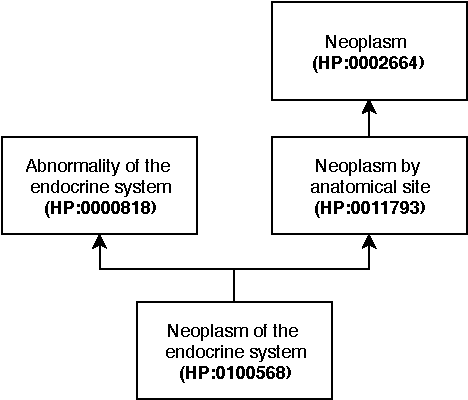
\includegraphics[width=10cm]{images/figure_1.pdf}
\fontsize{9}{10.8}\caption[HPO Ontology Excerpt]{An excerpt of the HPO ontology showing the first ancestors of \textit{neoplasm of the endocrine system}, using \textbf{is-a} relationships.}
\label{figure:1}
\end{figure}

The information provided by the ancestors is not expressed directly in the text and can support or disprove an identified relation. Ontologies are formally organized in machine-readable formats, facilitating their integration in relation extraction models. 

Using different sources of information, as additional data, to support automating searching for relations between biomedical concepts contributes to the development of pharmacogenomics, clinical trial screening, and adverse drug reaction identification \citep{10.1093/bib/bbx048}. Identifying new relations can help validate the results of recent research, and even propose new experimental hypotheses.

% ------------------------------> OBJECTIVES

\hypertarget{1.2}{\section{Objectives}}

The fundamental challenge of contemporary genetic analysis is correlating genes to their respective phenotypes. Existing systems that have the flexibility to be applied for the identification and extraction of human phenotype-gene relations, from biomedical literature, are scarce and limited. The main challenges that they face are the lack of annotated data sets; difficulties in the identification of phenotype entities, that are composed of multiple words, which makes name boundaries complex; and a scarcity of experts to perform curation of the identified relations. All of the aforementioned creates the need for automated corpora creation tools and the development of machine learning systems that can deal with the versatility of the gene and human phenotype entities and their relations, to better identify and extract them from text. Thus, the main goals of this work are:

\begin{enumerate}
\item{Create a large and versatile silver standard corpus of human phenotype-gene relations.}

\item{Develop a distantly supervised multi-instance learning module that combines a knowledge base for automatic extraction of human phenotype-gene relations (added to the IBRel system \citep{10.1371/journal.pone.0171929}).}

\item{Develop a deep learning module for automatic extraction of human phenotype-gene relations, taking advantage of domain-specific ontologies, like the Human Phenotype Ontology (HPO) and the Gene Ontology (added to the BO-LSTM system \citep{BOLSTM}).}
\end{enumerate}

First, the proposed pipeline should be able to generate a silver standard corpus based on articles dedicated to human phenotype-gene relations, using existing NER tools, and a gold standard relations knowledge base, provided by the HPO. Second, both machine learning systems (distantly supervised multi-instance learning, and deep learning) should be able to use the previous corpus to train a classifier and compare the classifications against a manually curated test-set.

The \textbf{hypothesis} of this dissertation is that information about human phenotype-gene relations can be efficiently extracted from biomedical literature using an automatically generated corpus, and machine learning techniques along with domain-specific ontologies.

% ------------------------------> METHODOLOGY

\section{Methodology}

The overall methods to accomplish the proposed objectives can be divided into three stages, one for each objective. The first stage is the creation of a silver standard human phenotype-gene relations corpus (generated in a fully automated manner) (Chapter \hyperlink{3}{3}), the second and third stages are the development of a distantly supervised multi-instance learning module that combines a knowledge base, and the development of a deep learning module that takes advantage of domain-specific ontologies, both for automatic extraction of human phenotype-gene relations (Chapter \hyperlink{4}{4}). 

To generate a silver standard for phenotype-gene relations, we need a pipeline that performs NER to recognize genes and human phenotype entities, and RE to extract and classify a relation between the identified human phenotype and gene entities. The first step is to gather abstracts using the PubMed API with manually defined keywords, namely, each gene name that participates in a relation (retrieved from a gold standard knowledge base of relations), \textit{homo sapiens}, and \textit{disease}. Then, the NER stage is performed using the Minimal Named-Entity Recognizer (MER) tool \citep{MER} to extract gene mentions, and the Identifying Human Phenotypes (IHP) tool \citep{IHP} to extract human phenotype mentions, from the abstracts. At last, using a gold standard relations knowledge base, provided by the HPO, the relations obtained by co-occurrence of the entities in the same sentence are marked \textit{Known} or \textit{Unknown}, and a subset (test-set) of the relations curated by domain experts. The \textit{Known} relations are in the knowledge base and the \textit{Unknown} relations are not yet identified or that do not exist.
The test-set was created by randomly selecting 260 relations to be reviewed by eight curators (50 relations each, with an overlap of 20 relations), all researchers working in the areas of Biology and Biochemistry.

While in the first stage a distant supervision approach is used to mark the relations with \textit{Known} or \textit{Unknown}, in the second stage the unlabeled silver standard corpus is going to be used to apply the distantly supervised multi-instance learning approach. These two distant supervision approaches differ in the way they are applied, as we are going to see in the following chapters.  

In the second stage, the goal is to use the corpus generated in the first stage unlabeled (annotated only with entity mentions) combined with a knowledge base (provided by the HPO), that provides examples for the relations we wanted to extract, to apply distantly supervised multi-instance learning. The best feature of this machine learning approach is the fact that it does not require the relations annotations, only the human phenotype and gene entities mentions, reducing the amount of manual effort necessary.

For the last stage, the main goal is to combine RNN (deep learning) algorithms with biological ontologies to improve the identification of human phenotype-gene relations in biomedical literature. Ontologies such as the HPO and the Gene Ontology provide a reliable representation of their respective domains and can be used as data representation layers to extract relations from text. The proposed system is going to represent each candidate pair as the sequence of the relations between the entities ancestors in their respective ontology and combine word embeddings and WordNet (generic English language ontology) to produce a model able to extract the \textit{Known} relations from text.

% ------------------------------> CONTRIBUTIONS

\hypertarget{1.4}{\section{Contributions}}

The main contribution of this dissertation was a feasible solution to identify and extract human phenotype-gene relations from text, that may be applied to other types of biomedical relations. This dissertation created the first corpus specific to human phenotype-gene relations, in an attainable and reproducible way, and two different system modules to extract these type of relations from highly heterogeneous text. Both the silver standard corpus and the developed modules evaluation was done with a test-set curated by domain experts. This section provides an overview of the contributions related to each of the objectives initially defined in Section \hyperlink{1.2}{1.2}. One contribution that did not corresponded to the initially defined goals was a book chapter presenting the base concepts for neural networks using ontologies for RE:

\begin{itemize}
    \item{\textbf{Book Chapter Submitted} \citep{book}: \textit{Using Neural Networks for Relation Extraction from Biomedical Literature for the book Artificial Neural Networks: Methods and Applications} (Diana Sousa, André Lamúrias, and Francisco M. Couto) in the Springer "Methods in Molecular Biology" series.}
\end{itemize}

% ----------------> OBJECTIVE 1

\subsection{Objective 1}

Chapter \hyperlink{3}{3} presents a pipeline to generate a silver standard human phenotype-gene relations corpus. The pipeline required the application of two NER tools and the availability of a list of gold standard relations. The evaluation of the corpus resorted to eight curators obtaining 87.01\% in precision with an inter-agreement of 87.58\%. The work developed for this objective resulted in one freely available silver standard corpus of human phenotype-gene relations\footnote{\url{https://github.com/lasigeBioTM/PGR}} and one paper accepted for the proceedings of an international conference (Core A):

\begin{itemize}
    \item{\textbf{Paper Accepted} \citep{DBLP:journals/corr/abs-1903-10728}: \textit{A Silver Standard Corpus of Human Phenotype-Gene Relations} (Diana Sousa, André Lamúrias, and Francisco M. Couto) in the Proceedings of the 2019 North American Chapter of the Association for Computational Linguistics.}
\end{itemize}

% ----------------> OBJECTIVE 2

\subsection{Objective 2}

Section \hyperlink{4.1.1}{4.1.1} presents a distantly supervised multi-instance learning module added to the IBRel system, to extract human phenotype-gene relations from text. The pipeline required a list of gold standard human phenotype-gene relations, the same as used in Chapter \hyperlink{3}{3}. The evaluation of the module resorted to the PGR test-set obtaining 73.48\% in F-measure. The work developed for this objective produced a high-performance distantly supervised multi-instance learning module that can effectively extract human phenotype-gene relations from text.

% ----------------> OBJECTIVE 3

\subsection{Objective 3}

Section \hyperlink{4.1.2}{4.1.2} presents a deep learning module added to the BO-LSTM system, able to extract human phenotype-gene relations from text. The pipeline required the ontologies available for both type of entities (HPO and Gene Ontology). These were added to the module as data representation layers to feed the deep learning model. The evaluation of the module resorted to the PGR test-set obtaining 55.00\% in F-measure. The work developed for this objective resulted in one journal publication (Q1 Scimago):

\begin{itemize}
    \item{\textbf{Paper Published} \citep{BOLSTM}: \textit{BO-LSTM: Classifying Relations Via Long
    Short-term Memory Networks Along Biomedical Ontologies} (André Lamúrias, \textbf{Diana Sousa}, Luka A. Clarke, and Francisco M. Couto) in BMC Bioinformatics.}
\end{itemize}

% ------------------------------> DOCUMENT STRUCTURE

\section{Document Structure}

Additionally to the present introductory chapter, this document is structured in four chapters as follows:

\begin{itemize}
   \item \textbf{Chapter \hyperlink{2}{2}} (Related Work) introduces the basic concepts and resources that support RE techniques, namely, Natural Language Processing (NLP), text mining primary tasks, initial approaches for RE, distant supervision for RE, neural networks for RE, and evaluation measures.
   \item \textbf{Chapter \hyperlink{3}{3}} (A Silver Standard Corpus of Phenotype-Gene Relations) presents the work developed to create a silver standard corpus of human phenotype-gene relations, including methods, evaluation, results and discussion.
   \item \textbf{Chapter \hyperlink{4}{4}} (Extracting Phenotype-Gene Relations) presents the system modules developed (distantly supervised multi-instance and deep learning modules) to accommodate human phenotype-gene RE, with methods, evaluation, results and discussion, for each module, and a detailed comparison between the two.
   \item \textbf{Chapter \hyperlink{5}{5}} (Conclusion) discusses the main conclusions of this work, and indicates some directions for future work.
\end{itemize}

\hypertarget{2}{}

\chapter{Related Work}

\rhead{Related Work}
\lhead{Chapter 2}

\vspace{-1.6cm}

% Gray Line
\begingroup
\color{gray}
\par\noindent\rule{\textwidth}{0.4pt}
\endgroup

\noindent{This chapter presents the basic concepts and resources that support Relation Extraction (RE) deep learning techniques, namely, Natural Language Processing (NLP), text mining primary tasks, initial approaches for RE, distant supervision for RE, neural networks for RE, and evaluation measures.}

% ------------------------------> NATURAL LANGUAGE PROCESSING

\hypertarget{2.1}{\section{Natural Language Processing}}

Natural Language Processing (NLP) is an area in computer science that aims to derive meaning from unstructured or highly heterogeneous text written by humans. NLP covers several techniques that constitute pre-processing steps for the tasks described in Section \hyperlink{2.2}{2.2}. These NLP techniques have different goals and are often combined to obtain higher performance.

\begin{itemize}

\item{\textbf{Tokenization}: has the purpose of breaking the text into tokens to be processed individually or as a sequence. These tokens are usually words but can also be phrases, numbers and other types of elements. The most straightforward form of tokenization is breaking the input text by whitespaces or punctuation. However, with scientific biomedical literature, that is usually descriptive and formal, we have to account for complex entities like human phenotype terms (composed of multiple words),  genes (represented by symbols), and other types of structured entities. These entities tend to be morphological complex and need specialized tokenization pipelines. Some researchers use a compression algorithm \citep{DBLP:journals/corr/SennrichHB15}, byte pair encoding (BPE), to account for biomedical vocabulary variability. BPE represents open vocabularies through a fixed-size vocabulary of variable-length character sequences, making it suitable for neural networks models, for instance.} 

\item{\textbf{Stemming and Lemmatization}: aims at reducing the variability of natural language by normalizing a token to its base form (stem) \citep{Manning:2008:IIR:1394399}. It can also take into account the context of the token, along with vocabulary and morphological analysis to determine the canonical form of the word (lemma). The stem can correspond only to a fragment of a word, but the lemma is always a real word. For instance, the stem of the word \textit{having} is \textit{hav} and the lemma is \textit{have}.}

\item{\textbf{Part-of-Speech Tagging}: consists of assigning each word of a sentence to the category where it belongs taking into account their context (e.g., verb or preposition). Each word can belong to more than one category. This feature is useful to gain information on the role of a word in a given sentence.}

\item{\textbf{Parse Tree}: represents the syntactic structure of a sentence. There are two different types of parse trees: constituency-based parse trees and dependency-based parse trees. The main difference between the two is that the first distinguishes between the terminal and non-terminal nodes and the second does not (all nodes are terminal). In constituency-based parse trees, each node of the tree is either a \textit{root} node, a \textit{branch} node, or a \textit{leaf} node. For each given sentence there is only one \textit{root} node. The \textit{branch} node connects to two or more \textit{child} nodes, and the \textit{leaf} node is terminal. These leaves correspond to the lexical tokens \citep{AHO}. Dependency-based parse trees are usually simpler because they only identify the primary syntactic structure, leading to fewer nodes. Parse trees generate structures that are used as inputs for other algorithms and can be constructed based on supervised learning techniques.}

\end{itemize}

% ------------------------------> TEXT MINING

\hypertarget{2.2}{\section{Text Mining Primary Tasks}}

Text mining has become a widespread approach to identify and extract information from unstructured or highly heterogeneous text \citep{10.1371/journal.pcbi.1005962}. Text mining is used to extract facts and relationships in a structured form that can be used to annotate specialized databases and to transfer knowledge between domains \citep{FLEUREN201597}. We may consider text mining as a sub-field of data mining. Thus, data mining algorithms can be applied if we transform text to a proper data representation, namely numeric vectors. Even if in recent years text mining tools have evolved considerably in number and quality, there are still many challenges in applying text mining to scientific biomedical literature. The main challenges are the complexity and heterogeneity of the written resources, which make the retrieval of relevant information, i.e., relations between entities, a non a trivial task.
Text Mining tools can target different tasks together or separately. Some of the primary tasks are Named Entity Recognition (NER), Named-Entity Linking (NEL) and Relation Extraction (RE).

\begin{itemize}

\item{\textbf{Named Entity Recognition (NER)}: seeks to recognize and classify entities mentioned in the text by identifying the offset of its first and last character. The workflow of this task starts by spliting the text in tokens and then labeling them into categories (part-of-speech (POS) tagging). Some tools that perform NER, used in this dissertation, are the Identifying Human Phenotypes tool (IHP) \citep{IHP} and the Minimal Named-Entity Recognizer tool (MER) \citep{MER} tools. IHP is a NER tool, specifically created to recognize HPO entities in unstructured text. It uses Stanford CoreNLP \citep{Manning2014} for text processing and applies Conditional Random Fields trained with a rich feature set, combined with hand-crafted validation rules and a dictionary to improve the recognition of human phenotypes. MER is a NER tool which given any lexicon or ontology (e.g., an OWL file) and an input text is able to return a list of recognized entities, their location, and links to their classes.}

\item{\textbf{Named-Entity Linking (NEL)}: maps the recognized entities to entries in a given knowledge base. For instance, a gene can be written in multiple ways and mentioned by different names or acronyms in a text. NEL links all these different nomenclatures to one unique identifier. There are several organizations dedicated to providing identifiers, among them the National Center for Biotechnology Information (NCBI)\footnote{\url{https://www.ncbi.nlm.nih.gov/}} for genes, and the Human Phenotype Ontology (HPO) \citep{HPO} for phenotypic abnormalities encountered in human diseases. Also, the HUGO Gene Nomenclature Committee (HGNC) at the European Bioinformatics Institute\footnote{\url{http://www.genenames.org/}} is responsible for approving unique symbols and names for human loci, including protein-coding genes, ncRNA genes, and pseudogenes, with the goal of promoting clear scientific communication. All approved symbols are stored in the HGNC database.}

\item{\textbf{Relation Extraction (RE)}: identifies relations between entities (recognized manually or by NER) in a text. Tools mainly consider relations by the co-occurrence of the entities in the same sentence, but some progress is being made to extend this task to the full document (taking into account a global context) \citep{Singhal2016TextMG}.}

\end{itemize}

The workflow of a typical RE system is presented in Figure \ref{figure:2}.

\begin{figure}[hbt!]
\captionsetup{font=small}
\centering
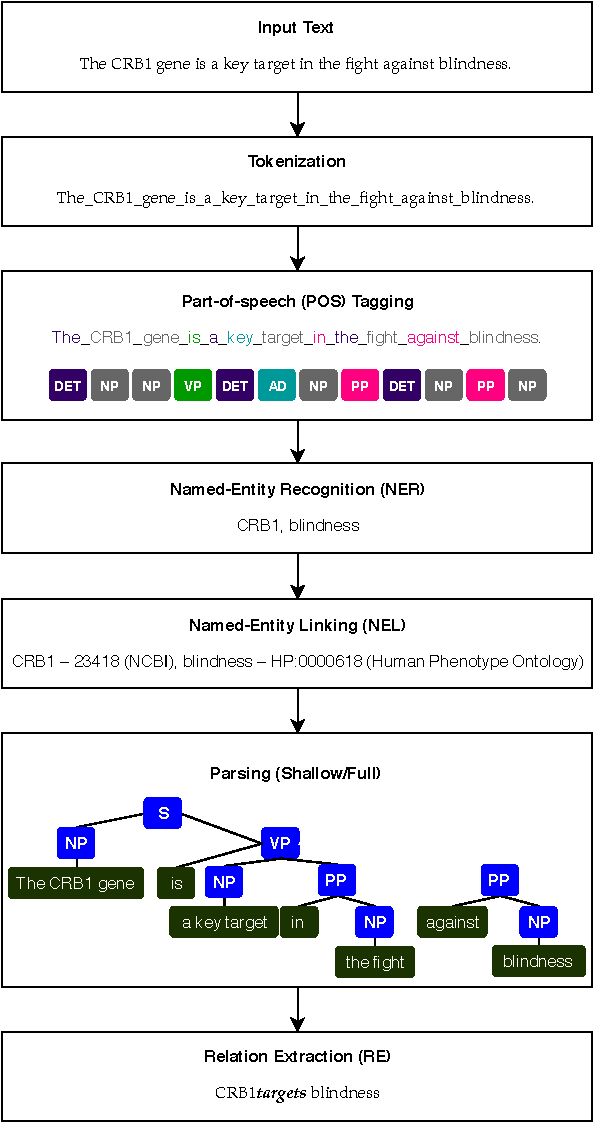
\includegraphics[width=9cm]{images/figure_2.pdf}
\fontsize{9}{10.8}\caption[Relation Extraction Workflow]{Workflow of a simplified RE system. \textbf{DET} is a determinant, \textbf{NP} is a noun, \textbf{VP} is a verb, \textbf{AD} is an adjective, and \textbf{PP} is a preposition. Text obtained from \cite{Alves2018}.}
\label{figure:2}
\end{figure}

% ------------------------------> INITIAL APPROACHES FOR RELATION EXTRACTION

\section{Initial Approaches for Relation Extraction}

Through the years, several approaches have been proposed to extract relations from biomedical literature \citep{10.1371/journal.pone.0171929}. Most of these approaches work on a sentence level to perform RE, due to the inherent complexity of biomedical literature.

\begin{itemize}

\item{\textbf{Co-occurrence}: assumes that if two entities are mentioned in the same sentence (co-occur), it is likely that they are related. Usually, the application of this approach results in a higher recall (most of the entities co-occurring in a sentence participate in a relation), and lower precision. Some methods use frequency-based scoring schemes to eliminate relations identified by chance \citep{10.1093/bib/bbm045}. Nowadays, most applications use co-occurrence as a baseline against more complex approaches \citep{bunescu-etal-2006-integrating}.}

\item{\textbf{Pattern-based}: uses manually defined and automatically generated patterns to extract relations. \textbf{Manually defined patterns} require domain expertise knowledge about the type of biomedical entities, their interactions, and the text subject at hand. Initial systems made use of regular expressions to match word patterns that reflected a relation between two entities \citep{Zhou2008}, making use of a dictionary of words that express a relation, such as \textit{trigger} and \textit{stimulate}. Later systems introduce part-of-speech (POS) tagging, but this proven to be too naive, especially when applied to complex sentences, such as the ones that we typically find in biomedical literature \citep{10.1093/bioinformatics/bti493}. Opposite to the co-occurrence approaches, manually defined patterns frequently achieve high precision but tend to have poor recall. This approach does not generalize well, and therefore is difficult to apply to new unseen data. \textbf{Automatically generated patterns} encompass two main approaches, bootstrapping with \textit{seeds} \citep{10.1093/bioinformatics/btr155} and leveraging of the corpora \citep{Liu:2011:GES:2107691.2107717}. The bootstrapping method uses a small set of relations known as \textit{seeds} (e.g., gene-disease pairs). The first step is to identify the \textit{seeds} in the data set and map the relation pattern they describe. The second step is to try to apply the mapped patterns to the data set to identify new pairs of relations that follow the same construction. Finally, expanding the original set of relations by adding these new pairs. When repeating all previous steps, if no more pairs are found, the process ends. Some systems apply distant supervision techniques to keep track of the validity of the added patterns. Distant supervision uses existing knowledge base entries as gold standards to confirm or discard a relation. This method is susceptible to noisy patterns, as the original set of relations grows. On the other hand, the leveraging of the corpora method makes immediately use of the entire data set to generate the patterns.  This method requires a higher number of annotated relations and produces highly specific patterns, that are unable to match new unseen data. Automatically generated patterns can achieve a higher recall than manually defined patterns, but overall the noisy patterns continue damaging the precision. Nevertheless, there are a few efforts to reduce the number of noisy patterns \citep{Nguyen2010}.}

\item{\textbf{Rule-based}: also uses manually defined and automatically generated rules from the training data to extract relations. Depending on the systems, the differences between pattern-based and ruled-based approaches can be minor. Ruled-based approaches not only use patterns but also additional restraints to cover issues that are difficult to express by patterns, such as checking for the negation of the relations \citep{10.1093/bioinformatics/bti084}. Some ruled-based systems distance themselves from pattern-based approaches by replacing regular expressions with heuristic algorithms and sets of procedures \citep{Rinaldi:2007:MRP:1224550.1224593}. Similarly to pattern-based, ruled-based approaches tend to have poor recall, even though rules tend to be more flexible. The trade-off recall/precision can be improved using automatic methods for rule creation \citep{10.1136/amiajnl-2011-000776}.}

\item{\textbf{Machine Learning (ML)-based}: usually makes use of large annotated biomedical corpora (supervised learning) to perform RE. These corpora are pre-processed using NLP tools and then used to train classification models. Beyond Distant Supervision and Neural Networks, described in detail in Sections \hyperlink{2.4}{2.4} and \hyperlink{2.5}{2.5}, respectively, it is possible to categorize ML methods into two main approaches, Feature-based and Kernel-based. \textbf{Feature-based approaches} represent each instance (e.g., sentence) as a vector in an n-dimensional space. Support Vector Machines (SVM) classifiers tend to be used to solve problems of binary classification, and are considered \textit{black-boxs} because there is no interference of the user in the classification process. These classifiers can use different features that are meant to represent the data characteristics (e.g., shortest path, bag-of-words (BOW), and POS tagging) \citep{Kim2008DetectionOG}. \textbf{Kernel-based approaches} main idea is to quantify the similarity between the different instances in a data set by computing the similarities of their representations \citep{Giuliano06exploitingshallow}. Kernel-based approaches add the structural representation of instances (e.g., by using parse trees). These methods can use one kernel or a combination of kernels (e.g., graph, sub-tree (ST), and shallow linguistic (SL)).}

\end{itemize}

% ------------------------------> DISTANT SUPERVISION FOR RELATION EXTRACTION

\section{Distant Supervision for Relation Extraction}

Distant Supervision (or weak supervision) heuristically assigns labels to the data in the training corpus based on a provided knowledge base. This technique considers that a pair of entities in any sentence corresponding to a knowledge base entry is likely to describe a relation between those entities. For instance, in the sentence \textit{the \textbf{CRB1} gene is a key target in the fight against \textbf{blindness}}, the \textit{CRB1} and \textit{blindness} entities correspond to an entry in the gold standard human phenotype-gene relations knowledge base, provided by the HPO, and therefore we assume that these entities participate in a relation. This creates a large number of false positives, because not necessarily all sentences that mention an entity pair express the target relation \citep{jiang-etal-2018-revisiting}. Nevertheless, this allows us to use a training corpus of any size, an advantage that we do not have in supervised machine learning approaches, that require an annotated corpus. 

Distant supervision is not a viable RE system by its own, but the pseudo-relations inferred using this method can be used to train a classifier through machine learning algorithms \citep{10.1371/journal.pone.0171929}. 

% ----------------> MULTI-INSTANCE LEARNING

\hypertarget{2.4}{\subsection{Multi-instance Learning}}

\textbf{Multi-instance learning} \citep{Dietterich:1997:SMI:249678.249682} can solve some of the limitations of distant supervision. This supervised machine learning method uses labeled \textit{bags} instead of labeled instances. These \textit{bags} contain many instances and are suited for when there is a limited amount of knowledge of the labels. The simplest case of multi-instance learning is binary classification. In this case a \textit{bag} is labeled negative if all the instances in the \textit{bag} are negative and positive if at least one of the instances in the \textit{bag} is positive. Then, these labeled \textit{bags} are fed to a learning algorithm. The algorithm that is going to be used in this dissertation is the \textbf{sparse multi-instance learning (sMIL) algorithm} \citep{Bunescu:2007:MIL:1273496.1273510}. The instance-level ($x$) classifier $f(\overrightarrow{x};\theta)$, where $\theta$ corresponds to the parameters learned by the classifier, is learned by using a set of instances $I = I^+ \cup I^-$ that we can define as follows \citep{AMORES201381}:

\begin{equation} \label{eq:negativeinstances}
\small
\begin{gathered}
I^+ = \{\mu(X) : X \in B^+\} \\
I^- = \{\overrightarrow{x} : \overrightarrow{x} \in B^-\}
\end{gathered}
\end{equation}

where $I^+$ and $I^-$ are the sets of instances considered positive and negative, respectively. $\mu(X)$ is the average of instances inside $X$, and $B^+$ and $B^-$ are the sets of positive and negative \textit{bags}, respectively.

The idea of the sMIL algorithm is to learn a classifier with a relaxed constraint on the classification of the positive instances in $I^+$. The goal is to avoid forcing the classifier to provide a positive value for all the instances of a positive \textit{bag} but only to at least one of the instances. To achieve this, the sMIL algorithm applies two sets of constraints:

\begin{equation} \label{eq:firstset}
\small
f(\overrightarrow{x};\theta) \leq -1 + \xi_-, \quad \forall \overrightarrow{x} \in I^-
\end{equation}

Equation \ref{eq:firstset} forces the $f(\overrightarrow{x};\theta)$ function to provide a negative value when applied to negative instances, allowing for some degree of misclassification with the $\xi_-$ variable. 

\begin{equation} \label{eq:secondset}
\small
f(\mu(X);\theta) \geq \bigg(\frac{2}{\mid X \mid} -1\bigg) - \xi_+, \quad \forall X \in B^+
\end{equation}

Equation \ref{eq:secondset} provides a more relaxed condition for positive instances, depending on the size of the \textit{bag} $X$ from where $\mu(X)$ is extracted. If the \textit{bag} $X$ only contains one instance, we use the standard condition $f(\mu(X);\theta) \geq  1 - \xi_+$ (maintaining the slack variable, $\xi_+$). Else, if the \textit{bag} $X$ contains many instances, the threshold imposed on the classifier is gradually more and more relaxed. 

The sMIL algorithm assumes that the positive \textit{bags} are sparse. An abstract may mention each entity in the candidate pair multiple times, but due to the limitation of the number of words the relation is usually stated only once. Non-biomedical RE systems already applied similar techniques to extract Freebase relations from newspaper articles \citep{10.1007/978-3-642-15939-8_10}, and to reduce the number of incorrectly labeled relations (by distant supervision methods) \citep{min-etal-2013-distant}.

% ------------------------------> NEURAL NETWORKS FOR RELATION EXTRACTION

\hypertarget{2.5}{\section{Neural Networks for Relation Extraction}}

Artificial neural networks have multiple different architectures implementations and variants. They often use data representations as additional sources of information to perform text mining tasks, and can even use ontologies as external sources of information to enrich the model.

% ----------------> ARCHITECTURES

\subsection{Architectures}

\textbf{Artificial Neural Networks} are a parallel combination of small processing units (nodes) which can acquire knowledge from the environment through a learning process and store the knowledge in the connections between the nodes \citep{Haykin:1998:NNC:521706} (represented by direct graphs \citep{GURESEN2011426}) (Figure \ref{figure:3}). The process is inspired by the biological brain function, having each node corresponding to a \textit{neuron} and the connections between the nodes representing the \textit{synapses}.

\begin{figure}[hbt!]
\captionsetup{font=small}
\centering
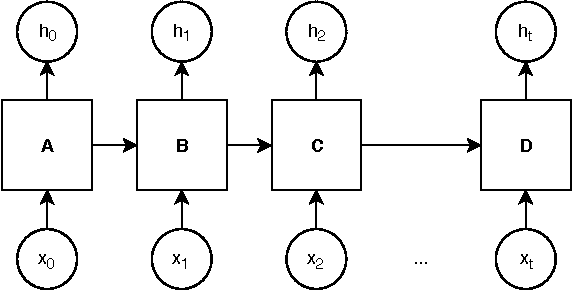
\includegraphics[width=10cm]{images/figure_3.pdf}
\fontsize{9}{10.8}\caption[Artificial Neural Networks Architecture]{Architecture representation of an artificial neural networks model, where x\textsubscript{0-t} represents the inputs and h\textsubscript{0-t} the respective outputs, for each module from A to D.}
\label{figure:3}
\end{figure}

\textbf{Recurrent Neural Networks} (RNN) is a type of artificial neural network where the connections between the nodes are able to follow a temporal sequence. This means that RNN can use their internal state, or \textit{memory}, to process each input sequence (Figure \ref{figure:4}). Deep learning techniques, such as RNN, aim to train classification models based on word embeddings, part-of-speech (POS) tagging, and other features. RNN classifiers have multilayer architectures, where each layer learns a different representation of the input data. This characteristic makes RNN classifiers flexible to multiple text mining tasks, without requiring task-specific feature engineering.

\begin{figure}[hbt!]
\captionsetup{font=small}
\centering
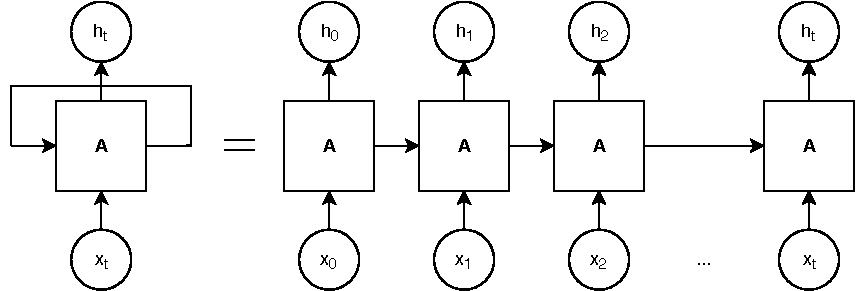
\includegraphics[width=13cm]{images/figure_4.pdf}
\fontsize{9}{10.8}\caption[Recurrent Neural Networks Architecture]{Architecture representation of a recurrent neural networks model, where x\textsubscript{0-t} represents the inputs and h\textsubscript{0-t} the respective outputs, for the repeating module A.}
\label{figure:4}
\end{figure}

\textbf{Long Short-Term Memory} (LSTM) networks are an alternative to regular RNN \citep{Hochreiter:1997:LSM:1246443.1246450}.  LSTMs are a type of RNN that handles long dependencies (e.g., sentences), making this classifier more suitable for the biomedical domain, where sentences are usually long and descriptive (Figure \ref{figure:5}). In recent years, the use of LSTMs to perform Relation Extraction (RE) tasks has become widespread in various domains, such as semantic relations between nominals \citep{miwa-bansal-2016-end}. \textbf{Bidirectional LSTMs} use two LSTM layers, at each step, one that reads the sentence from right to left, and other that reads from left to right. The combined output of both layers produces a final score for each step. Bidirectional LSTMs have yield better results than traditional LSTMs when applied to the same data sets \citep{zhang-etal-2015-bidirectional}.

\begin{figure}[hbt!]
\captionsetup{font=small}
\centering
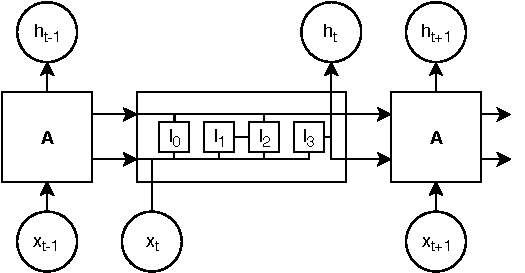
\includegraphics[width=10cm]{images/figure_5.pdf}
\fontsize{9}{10.8}\caption[Long Short-Term Memory Networks Architecture]{Architecture representation of a long-short-term memory networks model, where x\textsubscript{0-t} represents the inputs and h\textsubscript{0-t} the respective outputs, for the repeating module A, where each repeating module has four interacting layers (l\textsubscript{0-3}).}
\label{figure:5}
\end{figure}

% ----------------> DATA REPRESENTATIONS

\hypertarget{2.5.2}{\subsection{Data Representations}}

The combination of multiple and different language and entity related data representations is vital for the success of neural network models dedicated to RE tasks. Some of these features were already described in Section \hyperlink{2.1}{2.1}, such as POS tagging and parse trees. 

\textbf{Shortest Dependency Path} (SDP) is a feature that identifies the words between two entities mentioned in the text, concentrating the most relevant information while decreasing noise \citep{xu-etal-2015-classifying}. 

\textbf{Word Embeddings} are fixed-sized numerical vectors that aim to capture the syntactic and semantic word relationships. These word vectors models use multiple different pre-training sources, for instance, Word2Vec \citep{Mikolov:2013:DRW:2999792.2999959} uses English Wikipedia, and BERT \citep{BERT} uses both English Wikipedia and BooksCorpus. Early models, such as Word2Vec, learned one representation per word, but this proved to be problematic due to polysemous and homonymous words. Recently, most systems started to apply one embedding per word sense. One of the reasons why BERT outperforms previous methods is because it uses contextual models, meaning that it generates a unique representation for each word in a sentence. For instance, in the sentences fragments, \textit{they got \textbf{engaged}}, and \textit{students were very \textbf{engaged} in}, the word \textit{engaged} for non-contextual models would have the same meaning. BERT also outperforms other word vector models that take into account the sentence context, such as ELMo \citep{DBLP:journals/corr/abs-1802-05365} and ULMFit \citep{howard-ruder-2018-universal}, due to being an unsupervised and deeply bidirectional pre-trained language representation. 

\textbf{WordNet Hypernyms} are a feature that helps to hierarchize entities, structuring words similar to direct acyclic graphs \citep{WORDNET}. For example, \textit{vegetable} is a hypernym of \textit{tubers}, which in turn constitutes a hyponym of \textit{vegetable}. This feature is comparable to an ontology in the sense that a hierarchy relation is identified, but is missing the identification of the relations between the different terms. 

Using different features as information sources feeding individual channels leads to multichannel architecture models. Multichannel approaches were already proven to be effective in RE tasks \citep{xu-etal-2015-classifying}. 

Regarding biomedical RE, LSTMs were successful in identifying drug-drug interactions \citep{Wang2017}, gene-mutation relations \citep{song-etal-2018-n}, drug-mutation relations \citep{peng-etal-2017-cross}, among others. Some methods use domain-specific biomedical resources to train features for biomedical tasks. BioBERT \citep{BIOBERT} is a domain specific language representation model pre-trained on large-scale biomedical corpora, based on BERT \citep{BERT} architecture. BioBERT, using minimal task-specific architecture modifications, significantly outperforms previous biomedical state-of-the-art models in the text mining primary tasks of Named-Entity Recognition, Named-Entity Linking, and RE. The BR-LSTM \citep{Xu2018LeveragingBR} model uses a multichannel approach with pre-trained medical concept embeddings. Using the Unified Medical Language System (UMLS) concepts, BR-LSTM applies a medical concept embedding method developed by \cite{DeVine:2014:MSS:2661829.2661974}. BO-LSTM \citep{BOLSTM} uses the relations provided by domain-specific ontologies to aid the identification and classification of relations between biomedical entities in biomedical literature. 

% ----------------> ONTOLOGIES

\subsection{Ontologies}

An ontology is a structured way of providing a common vocabulary in which shared knowledge is represented \citep{Gruber}. Word embeddings can learn how to detect relations between entities but manifest difficulties in grasping the semantics of each entity and their specific domain. Domain-specific ontologies provide and formalize this knowledge. Biomedical ontologies are usually structured as a directed acyclic graph, where each node corresponds to an entity and the edges correspond to known relations between those entities. Thus, a structured representation of the semantics between entities and their relations, an ontology, allows us to use it as an added feature to a machine learning classifier. Some of the biomedical entities structured in publicly available ontologies are genes properties/attributes (Gene Ontology (GO)), phenotypes (Human Phenotype Ontology (HPO)), diseases (Disease Ontology (DO)), and chemicals (Chemical Entities of Biological Interest (ChEBI)). All of these entities participate in relations with different and same domain type entities. Hence, the information about each entity on a semantic level adds a new layer of knowledge to increase the performance of RE classifiers. For that end, this work uses the HPO and GO ontologies. The \textbf{HPO} is responsible for providing a standardized vocabulary of phenotypic abnormalities encountered in human diseases, using biomedical literature \citep{HPO}. The goal of this ontology is to facilitate medical documents readiness and exchange of medical information between medical professionals and researchers. The HPO entities are often long and descriptive, not following a specific nomenclature, making it hard to identify in unstructured text. The HPO currently contains over 13.000 terms and over 156.000 annotations to hereditary diseases. The \textbf{GO} defines a universe of concepts regarding gene functions (GO terms) and their relations \citep{GO}. The GO encompass three categories (sub-ontologies): \textit{molecular function} (11.110 terms), \textit{cellular component} (4.206 terms), and \textit{biological process} (29.687 terms), and three types of relations, \textit{is a}, \textit{part of} and \textit{regulates}. As in HPO terms, GO terms are usually long and descriptive. The primary goal of this ontology is to create a dynamic controlled vocabulary that can be applied to all eukaryotes, allowing for inferences regarding gene function by connecting different organisms.

Non-biomedical models using ontologies as an added source of information to neural networks is becoming widespread for several tasks. \cite{10.1007/978-3-319-50496-4_19} propose using word sense definitions, provided by the WordNet ontology, to learn one embedding per word sense for word sense disambiguation tasks. \cite{10.1007/978-3-319-63579-8_15} focus their work on semantic relations between ontologies and documents, using the DBpedia ontology. Some researchers explored graph embedding techniques \citep{GOYAL201878} that convert relations to a low dimensional space which represents the structure and properties of the graph. Other researchers have combined different sources of information, including ontological information, to do multi-label classification \citep{Kong:2013:MCM:2487575.2487577} and used ontology concepts to represent word tokens \citep{dasigi-etal-2017-ontology}.

However, few authors have used biomedical ontologies to perform RE. Textpresso \citep{10.1371/journal.pbio.0020309} is a text-mining system that works as a search engine of individual sentences, acquired from the full text of scientific articles, and articles. It integrates biomedical ontological information (e.g., of genes, phenotypes, and proteins) allowing for article and sentence search a query by term. The integration of the ontological information allows for semantic queries. This system helps database curation by automatically extracting biomedical relations. The IICE \citep{Lamurias2014IdentifyingIB} system uses kernel-based support vector machines along with an ensemble classifier to identify and classify drug-drug interactions, linking each chemical compound to the ChEBI ontology. \cite{Tripodi2017KnowledgeBaseEnrichedRE} system focus on drug-gene/protein interaction discovery to aid database curation, making use of ChEBI and GO ontologies. BO-LSTM \citep{BOLSTM} is the only model until now that incorporates ancestry information from biomedical ontologies with deep learning to extract relations from the text, specifically drug-drug interactions and gene-phenotype relations. 

% ------------------------------> EVALUATION MEASURES

\hypertarget{2.4}{\section{Evaluation Measures}}

The evaluation of machine learning systems is done by applying the trained models to a gold standard test-set, manually curated or annotated by domain experts and unseen by the system. For a Relation Extraction (RE) task, the gold standard test-set should correspond to the list of pairs of entities (e.g., phenotype-gene or gene-disease pairs) that co-occur in the same sentences and their relation (\textit{Known} or \textit{Unknown}).
To any given information extraction system it is necessary to define what constitutes a positive and negative result. In RE tasks the types of results possible are shown in Table \ref{table:evaluation}.

\begin{table}[!ht]
\renewcommand\arraystretch{1.2}
\small
\captionsetup{font=small}
\caption[Types of Results Obtained with an Information Extraction System for a RE Task]{Types of results obtained with an information extraction system for a RE task.}
\centering
\taburulecolor{black}
\begin{tabular}{ |c|c|c| }
\hline
\textbf{Annotator (Gold Standard)} & \textbf{System} & \textbf{Classification}\\
\hline\hline
\multirow{2}{*}{Relation} & Relation & True Positive (TP) \\
\cline{2-3}
 & No Relation & False Negative (FN) \\ 
\hline
\multirow{2}{*}{No Relation} & Relation & False Positive (FP) \\
\cline{2-3}
 & No Relation & True Negative (TN) \\
 \hline
\end{tabular}
\label{table:evaluation}
\end{table}

The primary goal of a given information retrieval system is to maximize the number of TP and TN. To compare results obtained with different data sets or different tools we have three distinct evaluation metrics: recall, precision and F-measure. Precision represents how often the results are correct, recall the number of correct results identified and F-measure is a combination of both metrics to express overall performance, being the harmonic mean of precision and recall:

\begin{equation}
\small
Recall = \frac{TP}{TP + FN}
\qquad
Precision = \frac{TP}{TP + FP}
\qquad
F-measure = \frac{2\times Precision\times Recall}{Precision + Recall}
\label{equation:evaluation}
\end{equation}

The performance of the most recent systems dedicated to biomedical RE, described in Section \hyperlink{2.5.2}{2.5.2}, is shown in Table \ref{table:evaluation_soa}. These systems are not comparable, since each system is focused on the relations between different biomedical entities, and even addresses more than binary relations, such as the Graph LSTM (GOLD) system. 

\begin{table}[!ht]
\renewcommand\arraystretch{1.2}
\small
\captionsetup{font=small}
\caption[Biomedical RE Systems Performance]{Biomedical RE systems current performance.}
\centering
\taburulecolor{black}
\begin{tabular}{ |c|c|c|c| }
\hline
\textbf{System} & \textbf{Precision} & \textbf{Recall} & \textbf{F-Measure}\\
\hline\hline
DLSTM \citep{Wang2017} & 0.7253 & 0.7149 & 0.7200 \\
\hline
Graph LSTM (GOLD) \citep{song-etal-2018-n} & 0.4330 & 0.3050 & 0.3580 \\ 
\hline
BioBERT \citep{BIOBERT} & 0.8582 & 0.8640 & 0.8604 \\
\hline
BR-LSTM \citep{Xu2018LeveragingBR} & 0.7152 & 0.7079 & 0.7115 \\
\hline
BO-LSTM \citep{BOLSTM} & 0.6572 & 0.8184 & 0.7290 \\
\hline
\end{tabular}
\label{table:evaluation_soa}
\end{table}

For RE tasks a human acceptable performance is usually around 85/90\% in F-measure \citep{Aroyo2015TruthIA}. To facilitate the creation of gold standards we should strive for semi-automation, that is, employ automatic methods for corpora annotation (creating silver standard corpora), and then correct those annotations using domain-specific curators. 

The inter-curator agreement metric, that is going to be used in this work to evaluate the quality of the curation of the silver standard corpus annotations, is calculated through the Cohen's Kappa Coefficient (κ) \citep{doi:10.1177/001316446002000104}:

\begin{equation}
\small
\kappa = \frac{P(A) - P(E)}{1 - P(E)}
\label{equation:agreement}
\end{equation}

where \textit{P}(\textit{A}) corresponds to the percentage of agreement and \textit{P}(\textit{E}) the percentage that was expected inter-curators or inter-annotators to agree by chance.


\hypertarget{3}{}

\chapter{Methodology}

\rhead{Methodology}
\lhead{Chapter 3}

\vspace{-1.6cm}

% Gray Line
\begingroup
\color{gray}
\par\noindent\rule{\textwidth}{0.4pt}
\endgroup

%In order to achieve the objectives proposed in Section 1.2, i.e., the development of a recommender system suitable for Large-Scale Scientific Datasets, we will follow the methodology represented in Figure 4.1. Since this is a complex project with several phases, we divided the methodology in tasks. Each task, as well as their respective challenges and proposed solutions, are described below.
\noindent{This section will present a modular description of the deep learning system for biomedical Relation Extraction (RE) combining external sources of knowledge (regarding main objectives 1 and 2). Also, the overall evaluation process and particularities of the biomedical case studies (objective 3). Finally, the last subsection will present the project planning according to a timeline regarding the three main objectives' specificities.} 


\section{System}

The modular description is a representation of what is going to be tested, especially regarding the integration of pre-existing word embeddings and semantics for RE, since the plan is to analyse multiple approaches (Section \hyperlink{2.2}{2.2}) to access the most efficient. The complete flowchart of the system is illustrated in Figure \ref{flow}. Each step is described in more detail in the following enumeration:

\begin{figure}
\centering
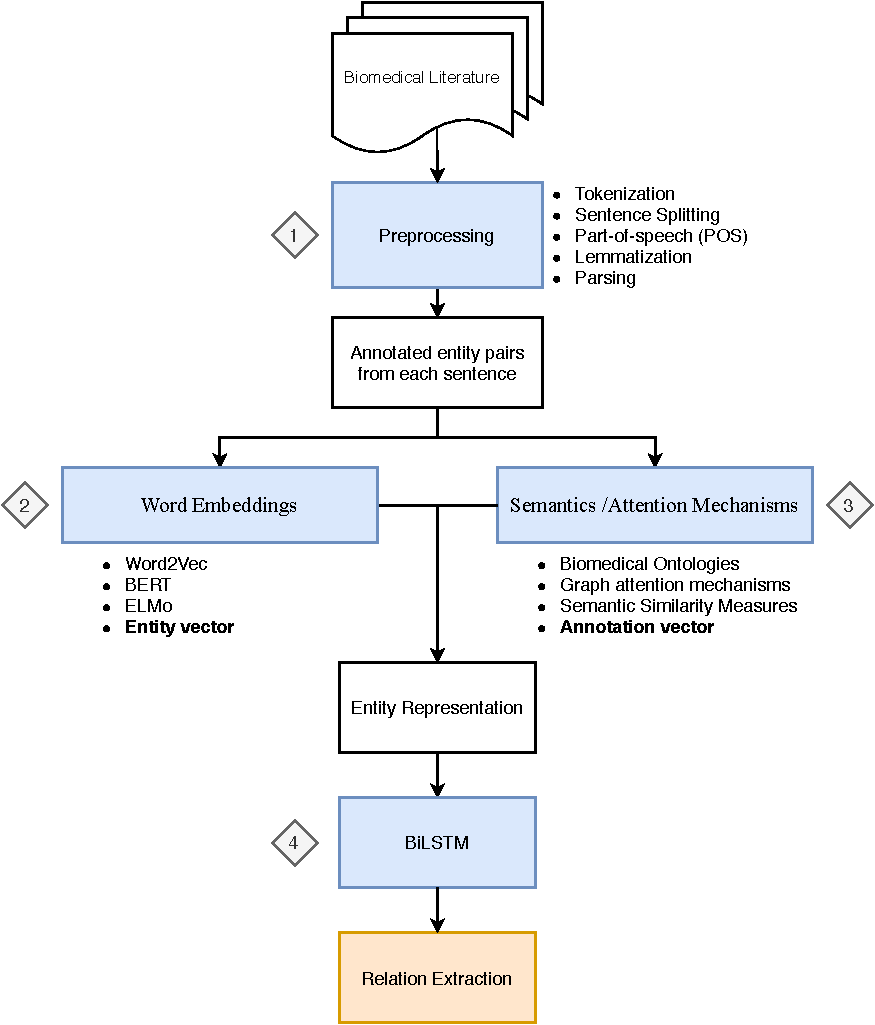
\includegraphics[width=15.5cm]{images/flowchart.pdf}
\caption[Flowchart Illustrating Proposed System]{Flowchart illustrating the proposed deep learning system for biomedical relation extraction combining external sources of knowledge, with the numbered main steps.}
\label{flow}
\end{figure}

\begin{enumerate}
    \item  \textbf{Preprocessing} The preprocessing step will encompass tokenization, sentence splitting, part-of-speech (POS) tagging, lemmatization, and parsing. Each set of biomedical entities has distinct textual characteristics, inherent to unique contexts. Each entity will be identified with a domain-specific Named-Entity Recognition (NER) system \citep{yadav2019survey}. Regarding Named-Entity Linking (NEL), entities such as genes, chemicals, diseases, and proteins, will be matched to an identifier through the corresponding ontology. These tasks need to be optimized to perform RE.   
    \item \textbf{Word Embbeddings} Recurrent Neural Networks (RNN) train classification models based on word embeddings and other features. This system is going to incorporate different state-of-the-art word embeddings like Word2Vec \citep{li2017neural}, ELMo \citep{peters2018deep} and BERT \citep{lin2016neural}, and make use of different combinations of channels to maximize performance.
    \item \textbf{Semantics/Attention Mechanisms} Taking advantage of semantics can provide supplementary information that may not be present in the training data. Ontologies formalize existing knowledge about entities such as genes \citep{ashburner2000gene}, and diseases \citep{schriml2012disease}. Through representation of each entity as the sequence of its ancestors, it is possible to detect new relations between entities that were not evident by only using the training data. Also, a new word embedding layer is going to be built taking advantage of semantics/attention mechanisms. Word embeddings usually represent a variable length sentence into a fixed length vector, where each element of the vector encodes some semantics of the original sentence. The innovation resides in adding the ontology semantics of the identified entity to each vector, as well a graph attention mechanism, and test the use of semantic similarity measures. For example, if the \textit{BRCA1} gene is semantically similar to the \textit{BRAF} gene and the \textit{BRCA1} has an established relation with the \textit{tumor} phenotype, it could be possible to infer that \textit{BRAF} gene also has a relation with the \textit{tumor} phenotype, even if that is not evident by the training data.
    \item \textbf{BiLSTM} The RE system between the linked identified entities is going to be built using bidirectional Long Short-Term Memory (LSTM) networks, a deep learning method that deals with long sentences of words, with a similar architecture to RNN, based on the work of \cite{lamurias2019bo} (BO-LSTM system). These models use different types of information, known as channels, such as word embeddings, part-of-speech tags, grammatical relations, and WordNet hypernyms \citep{ciaramita2006broad}. Each of these channels has different types of input information and is responsible for one of the model layers. All of these layers can be connected to a softmax layer outputting the probabilities of each class. 
\end{enumerate}

\section{Evaluation}

The evaluation of deep learning based systems is done by applying the trained models to a gold standard, manually curated by domain experts and unseen by the information extraction system. To compare results obtained with different datasets or different tools we have three distinct state-of-the-art evaluation metrics: recall, precision, and F-measure.

\begin{enumerate}
    \item Evaluation of the integrated system on different benchmark datasets: The developed systems will use benchmark datasets, such as the semantic relations between pairs of nominals corpus SemEval-2010 Task 8 \citep{hendrickx2010semeval}, the drug-drug interactions corpus SemEval-2013 task-9 \citep{segura2013semeval}, and the Phenotype-Gene Relations corpus \citep{sousa2019silver}.
    \item Development of an improved automated corpus creation based on the PGR corpus for system assessment \citep{sousa2019silver}: Improving automating corpus creation is of interest to create training data for the developed systems since some biomedical relations do not have gold standard corpus available to use to test the quality of these systems. Leveraging on previous work \citep{sousa2019silver} it is possible to generate multiple silver standard corpus for different entities with good enough results. These results have been demonstrated to be sufficient for training deep learning-based systems.
    \item  Application of the systems to other fields and to different languages: Apply domain-specific ontologies of non-biomedical topics, for example, the Planteome, a plant ontology \citep{cooper2018planteome}, using benchmark datasets. Also, making use of the translation of some ontologies like the HPO, and the DECS ontology \citep{campanatti2010health} (i.e., Health Sciences Descriptors in Portuguese and Spanish) linked to English mesh terms \citep{papagiannopoulou2016large}, will allow us to study the effect of different languages in the system.
    \item Participation in different competitions such as SemEval, BioCreative, and BioASQ \citep{huang2016community}.
\end{enumerate}

\section{Case Studies}

The case studies of this project are going to be human phenotypic abnormalities and the identification of cancer-nutrition interactions regarding our collaboration with the World Health Organization (WHO). There is no RE deep learning system that uses the knowledge from the HPO \citep{robinson2010human} to extract relevant clinical information.

Human phenotype terms often have more than one word, are descriptive, and do not follow a specific nomenclature. The individual features of these terms and the subcategory of cancer-related phenotypes will be studied to resolve the preprocessing step and identify the most appropriate semantic additions to the system.  

Through these methods, it will be possible to identify new relation candidates for gold standard knowledge bases of both relations between human phenotype entities and other biomedical entities and cancer-nutrition interactions. Thus, the system will be able to train models using pre-existing datasets to identify new relations between human phenotypes and other biomedical entities and cancer-nutrition interactions.

\section{Planning}

The thesis project encompasses three main objectives, related to deep learning, semantics, and their application to the biomedical domain. Some of the sub-objectives may overlap, and implementation and assessment will continuously incorporate the software developed in the previous steps.

Figure \ref{figure:timeline} presents the timeline of the objectives and sub-objectives of the thesis.

\begin{landscape}

\begin{figure}
\captionsetup{font=small}
\centering
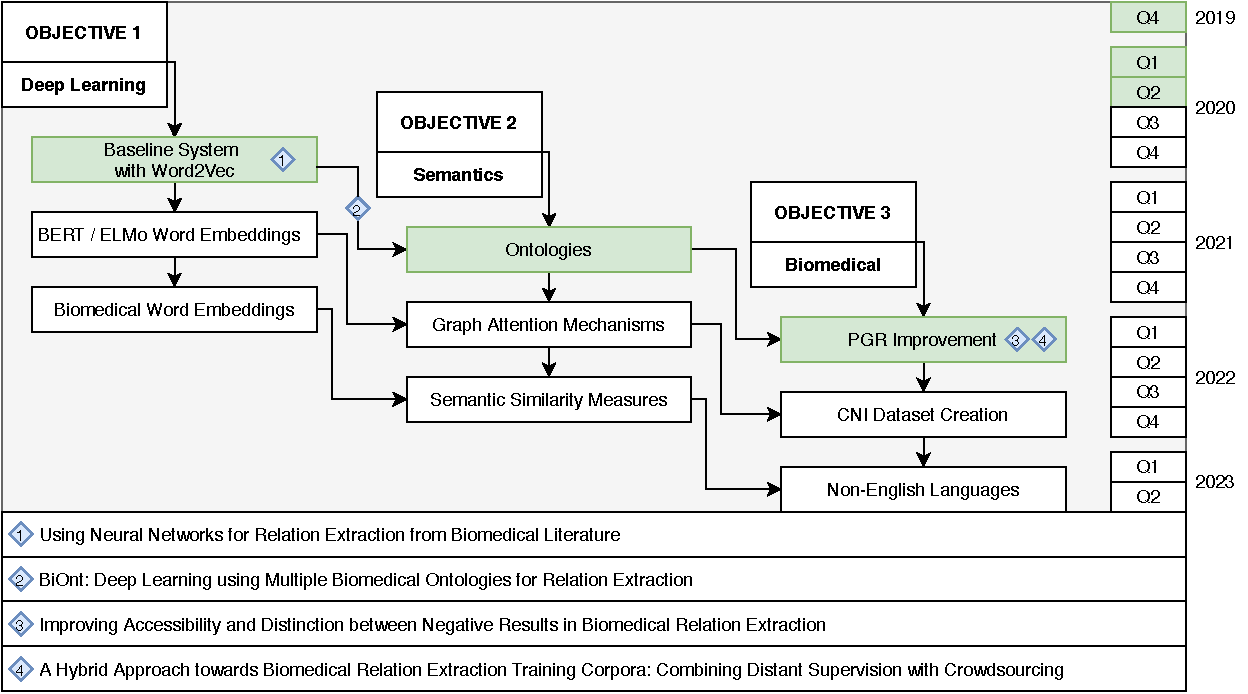
\includegraphics[width=20cm]{images/timeline.pdf}
\fontsize{9}{10.8}\caption[Thesis Project Timeline]{Project timeline. Main objectives and sub-objectives of the thesis. In green, the sub-objectives already fulfilled (according to the timeline). Identified with 1, 2, 3, and 4 are the articles published (1-3) and submitted (4) and to what thesis step they refer. PGR stands for the Phenotype-Gene Relations dataset and CNI for cancer-nutrition interactions.}
\label{figure:timeline}
\end{figure}

\end{landscape}

\hypertarget{4}{}

\chapter{Work in Progress}

\rhead{Work in Progress}
\lhead{Chapter 4}

\vspace{-1.6cm}

% Gray Line
\begingroup
\color{gray}
\par\noindent\rule{\textwidth}{0.4pt}
\endgroup

\noindent{Some of the early contributions and work in progress of this project are stated in the following sections in the form of abstracts. All articles are fully available in the \hyperlink{a}{Appendix} section of this work. The articles are also present in the project timeline (Figure \ref{figure:timeline}).}

% ------------------------------> EARLY CONTRIBUTIONS

\section{State-of-the-art Survey}

This work's first contribution was a book chapter presenting the base concepts for neural networks using ontologies for RE, which corresponds to the necessary precedent steps towards the first sub-objective (Baseline System with Word2Vec) is identified in Figure \ref{figure:timeline} as \textbf{1}:

\begin{itemize}
    \item{\textbf{Book Chapter to Publish August 2020} \citep{sousa2019using} (\hyperlink{AA}{Appendix A}): \textit{Using Neural Networks for Relation Extraction from Biomedical Literature for the book Artificial Neural Networks: Methods and Applications} (Diana Sousa, Andre Lamurias, and Francisco M. Couto) in the Springer "Methods in Molecular Biology" series.}
\end{itemize}

\subsection{Abstract}

Using different sources of information to support automated extracting of relations between biomedical concepts contributes to the development of our understanding of biological systems. The primary comprehensive source of these relations is biomedical literature. Several relation extraction approaches have been proposed to identify relations between concepts in biomedical literature, namely using neural networks algorithms. The use of multichannel architectures composed of multiple data representations, as in deep neural networks, is leading to state-of-the-art results. The right combination of data representations can eventually lead us to even higher evaluation scores in relation extraction tasks. Thus, biomedical ontologies play a fundamental role by providing semantic and ancestry information about an entity. The incorporation of biomedical ontologies has already been proved to enhance previous state-of-the-art results.


\section{Baseline Deep Learning System using Multiple Biomedical Ontologies}

Following the state-of-the-art survey, the next step was to develop a baseline system with Word2Vec (based on \cite{lamurias2019bo} work) and combine multiple biomedical ontologies to the system to test if there was added performance by the use of these knowledge graphs. These steps correspond to the first sub-objective of the Deep Learning objective, and the first subjective within the Semantics objective (in Figure \ref{figure:timeline} marked as \textbf{2}). The work developed for these steps resulted in a conference paper (Core A): 

\begin{itemize}
    \item{\textbf{Paper Published} \citep{sousa2020biont} (\hyperlink{AB}{Appendix B}): \textit{BiOnt: Deep Learning using Multiple Biomedical Ontologies for Relation Extraction} (Diana Sousa and Francisco M. Couto) in the European Conference on Information Retrieval.}
\end{itemize}

\subsection{Abstract}

Successful biomedical relation extraction can provide evidence to researchers and clinicians about possible unknown associations between biomedical entities, advancing the current knowledge we have about those entities and their inherent mechanisms. Most biomedical relation extraction systems do not resort to external sources of knowledge, such as domain-specific ontologies. However, using deep learning methods, along with biomedical ontologies, has been recently shown to effectively advance the biomedical relation extraction field. To perform relation extraction, our deep learning system, BiOnt, employs four types of biomedical ontologies, namely, the Gene Ontology, the Human Phenotype Ontology, the Human Disease Ontology, and the Chemical Entities of Biological Interest, regarding gene-products, phenotypes, diseases, and chemical compounds, respectively. We tested our system with three data sets that represent three different types of relations of biomedical entities. BiOnt achieved, in F-score, an improvement of 4.93\% points for drug-drug interactions (DDI corpus), 4.99\% points for phenotype-gene relations (PGR corpus), and 2.21\% points for chemical-induced disease relations (BC5CDR corpus), relatively to the state-of-the-art. The code supporting this system is available at \url{https://github.com/lasigeBioTM/BiOnt}. 


\section{PGR Improvement}

The next two early contributions refer to the first sub-objective (PGR Improvement) within the Biomedical objective (in Figure \ref{figure:timeline} marked as \textbf{3} and \textbf{4}). The first reflects the first steps toward identifying negative relations where there is a mention of no relation between two entities using the PGR dataset \citep{sousa2019silver}. The second contribution presents the work done regarding using the PGR dataset along with MTurk crowdsourcing services for dataset improvement. 

\subsection{Focusing on Negative Biomedical Relations}

This work was developed during the 6th Biomedical Linked Annotation Hackathon (BLAH6) and resulted in one journal publication:

\begin{itemize}
    \item{\textbf{Paper Published} \citep{sousa2020improving} (\hyperlink{AC}{Appendix C}): \textit{Improving Accessibility and Distinction between Negative Results in Biomedical Relation Extraction} (Diana Sousa, Andre Lamurias, and Francisco M. Couto) in Genomics \& Informatics.}
\end{itemize}

\subsubsection{Abstract}

Accessible negative results are relevant for researchers and clinicians not only to limit their search space but also to prevent the costly re-exploration of research hypotheses. However, most biomedical relation extraction datasets do not seek to distinguish between a false and a negative relation among two biomedical entities. Furthermore, datasets created using distant supervision techniques also have some false negative relations that constitute undocumented/unknown relations (missing from a knowledge base). We propose to improve the distinction between these concepts, by revising a subset of the relations marked as false on the phenotype-gene relations corpus and give the first steps to automatically distinguish between the false (F), negative (N), and unknown (U) results. Our work resulted in a sample of 127 manually annotated FNU relations and a weighted-F1 of 0.5609 for their automatic distinction. This work was developed during the 6th Biomedical Linked Annotation Hackathon (BLAH6).


\subsection{Alling Distant Supervison to Crowdsourcing}

The work developed for this step resulted in one journal submission:

\begin{itemize}
    \item{\textbf{Paper Submitted} (\hyperlink{AD}{Appendix D}): \textit{A Hybrid Approach towards Biomedical Relation Extraction Training Corpora: Combining Distant Supervision with Crowdsourcing} (Diana Sousa, Andre Lamurias, and Francisco M. Couto).}
\end{itemize}

\subsubsection{Abstract}

Biomedical Relation Extraction (RE) datasets are vital in the construction of knowledge bases, and to potentiate the discovery of new interactions. There are several ways to create biomedical RE datasets, some more reliable than others, such as resorting to domain expert annotations. However, the emerging use of crowdsourcing platforms, such as Amazon Mechanical Turk (MTurk), can potentially reduce the cost of RE dataset construction, even if the same level of quality cannot be guaranteed. There is a lack of power of the researcher to control who, how, and in what context workers engage in crowdsourcing platforms. Hence, allying distant supervision with crowdsourcing can be a more reliable alternative. The crowdsourcing workers would be asked only to rectify or discard already existing annotations, which would make the process less dependent on their ability to interpret complex biomedical sentences. In this work, we use a previously created distantly supervised dataset of human phenotype-gene relations (PGR dataset) to perform crowdsourcing validation. We divided the original dataset into two annotation tasks: Task 1, 70\% of the dataset annotated by one worker, and Task 2, 30\% of the dataset annotated by seven workers. Also, for Task 2, we added an extra rater on-site and a domain expert, to further assess the crowdsourcing validation quality. Here, we describe a detailed pipeline for RE crowdsourcing validation, creating a new release of the PGR dataset with partial domain expert revision, and assess the quality of the MTurk platform. We applied the new dataset to two state-of-the-art deep learning systems (BiOnt and BioBERT) and compared its performance with the original PGR dataset, as well as combinations between the two, achieving 0.3494 average increase in F-measure. The code supporting our work and the new release of the PGR dataset will be made publicly available upon acceptance of this manuscript.



\hypertarget{5}{}

\chapter{Conclusion}

\rhead{Conclusion}
\lhead{Chapter 5}

\vspace{-1.6cm}

% Gray Line
\begingroup
\color{gray}
\par\noindent\rule{\textwidth}{0.4pt}
\endgroup



\noindent{The main way we communicate scientific knowledge is through scientific literature. At the current rate of document growth, the only way to process this amount of information is by using computational methods. The information obtained through these methods can lead to a better understanding of biological systems. However, as most learning models require a large amount of training data, applying these learning algorithms to biomedical text mining is often unsuccessful due to the lack of training data in biomedical fields. This work made an important contribution to overcame this issue by creating a large and versatile silver standard corpus, the Phenotype-Gene Relations (PGR) corpus. 

When creating biomedical text mining systems, it is essential to take into account the specific characteristics of biomedical literature. Biological information follows different nomenclatures and levels of complexity. The distantly supervised multi-instance and deep learning modules, developed in this work, were successfully built to accommodate the specificities of human phenotype and gene entities. Thus, this work accomplished the initial objectives (Section \hyperlink{1.2}{1.2}) with highly promising results, fulfilling the initial hypothesis (Section \hyperlink{1.2.1}{1.2.1}).}

Following the growing tendency of systems targeting different biomedical relations, there is an increasing need for more domain-specific corpora, that can only be accomplished by automated corpus creation. The PGR corpus consists of 1712 abstracts, 5676 human phenotype annotations, 13835 gene annotations, and 4283 relations\footnote{Query 1, corresponds to the \textit{10/12/2018} release of PGR}. Using Named-Entity Recognition tools and a distantly supervised approach it was possible to effectively identify and extract human phenotype and gene entities and their relations. These results were partially evaluated by eight curators, obtaining a precision of 87.01\%, with an inter-curator agreement of 87.58\%. The PGR corpus was made publicly available to the research community.\footnote{\url{https://github.com/lasigeBioTM/PGR}}

Automatic biomedical Relation Extraction (RE) still has a long way to go to achieve human-level performance scores. Over recent years, some innovative systems have successively achieved better results by making use of multiple knowledge sources and data representations. These systems not only rely on the training data but make use of different language and entity related features, to create models that identify relations in highly heterogeneous text. Although, even with an optimal combination of features and the ideal features to perform biomedical Relation Extraction (RE) tasks are still far from human level performance. Nevertheless, the results achieved by the distantly supervised multi-instance and deep learning modules developed in this dissertation, were respectively, 73.48\% and 55.00\% in F-measure. These modules were able to detect new gold standard relations that were not present in the reference knowledge base. 

This work showed that the knowledge encoded in biomedical ontologies and gold standard knowledge bases plays a vital part in the development of learning systems, providing semantic and ancestry information for entities, such as genes, proteins, phenotypes, and diseases. Also, it produced one freely available silver standard corpus of human phenotype-gene relations; a high-performance distantly supervised multi-instance learning module that can effectively extract human phenotype-gene relations from text; and one deep learning module with an ontological data representation layer (Section \hyperlink{1.4}{1.4}).

Integrating different knowledge sources instead of relying solely on the training data for creating classification models will allow us not only to find relevant information for a particular problem quicker, but also to validate the results of recent research, and propose new experimental hypotheses. 

This work produced three publications including a book chapter about neural networks, a journal paper describing the ontologies applications to deep learning systems, and a conference paper describing the creation of the PGR corpus.


% ------------------------------> FUTURE WORK

\section{Future Work}

For Chapter \hyperlink{3}{3}, future work can include manually correcting the human phenotype annotations that did not match any HPO identifier, with the potential of expanding the number of human phenotype annotations almost 2-fold and increasing the overall recall. Also, to expand the corpus by identifying more missed gene annotations using pattern matching, which is possible due to the approach being fully automated. Another possibility is the expansion of the test-set for more accurate capture of the variance in the corpus. For example, we can select a subset of annotated documents in which two curators could work to grasp the complexity of manually annotating some of these abstracts. Further, it is possible to use semantic similarity to validate the human phenotype-gene relations. Semantic similarity has been used to compare different types of biomedical entities \citep{SSM} and it is a measure of closeness based on their biological role. For example, if the \textit{BRCA1} gene is semantically similar to the \textit{BRAF} gene and the \textit{BRCA1} has an established relation with the \textit{tumor} phenotype, it could be possible to infer that \textit{BRAF} gene also has a relation with the \textit{tumor} phenotype, even if that is not evident by the training data. Finally, the effect of different NER systems applied to the pipeline should be studied.

Regarding the distantly supervised multi-instance learning module, the parameters of the miSVM package could be optimized using cross-validation on the PGR corpus, and different algorithms implemented (besides the sparse multi-instance learning (sMIL) algorithm \citep{Bunescu:2007:MIL:1273496.1273510}). 

For the deep learning module, it is possible to integrate the ontological information in different ways. For instance, one could consider only the relations between the ancestors with the highest information content (more relevant for the candidate pair they characterize). The information content could be inferred from the probability of each term in each ontology or resorting to an external data-set. Also, the already mentioned semantic similarity measurement could account for non-transitive relations (within the same ontology).

Future work may also consist in outperforming the BioBERT application by using their model along with a data representation layer of biomedical ontologies, given that this work already proved to improve the recall when comparing with an identical model that did not resort to ontological information.

Lastly, combining the techniques developed and presented throughout Chapters \hyperlink{3}{3} and \hyperlink{4}{4}, it would be useful to develop a software tool in which we could annotate documents with human phenotype and gene entities and their relations. More than that, to employ and adapt these techniques to other combinations of biomedical entities to further expand our knowledge about biological systems. 


\pagestyle{plain}  % no more header 

\newpage
\renewcommand\bibname{References}
\bibliography{references}
\bibliographystyle{apalike}



\chaptertitlefont{\LARGE}



\hypertarget{a}{\appendix}
\hypertarget{AA}{\chapter{Using Neural Networks for Relation Extraction from Biomedical Literature}}
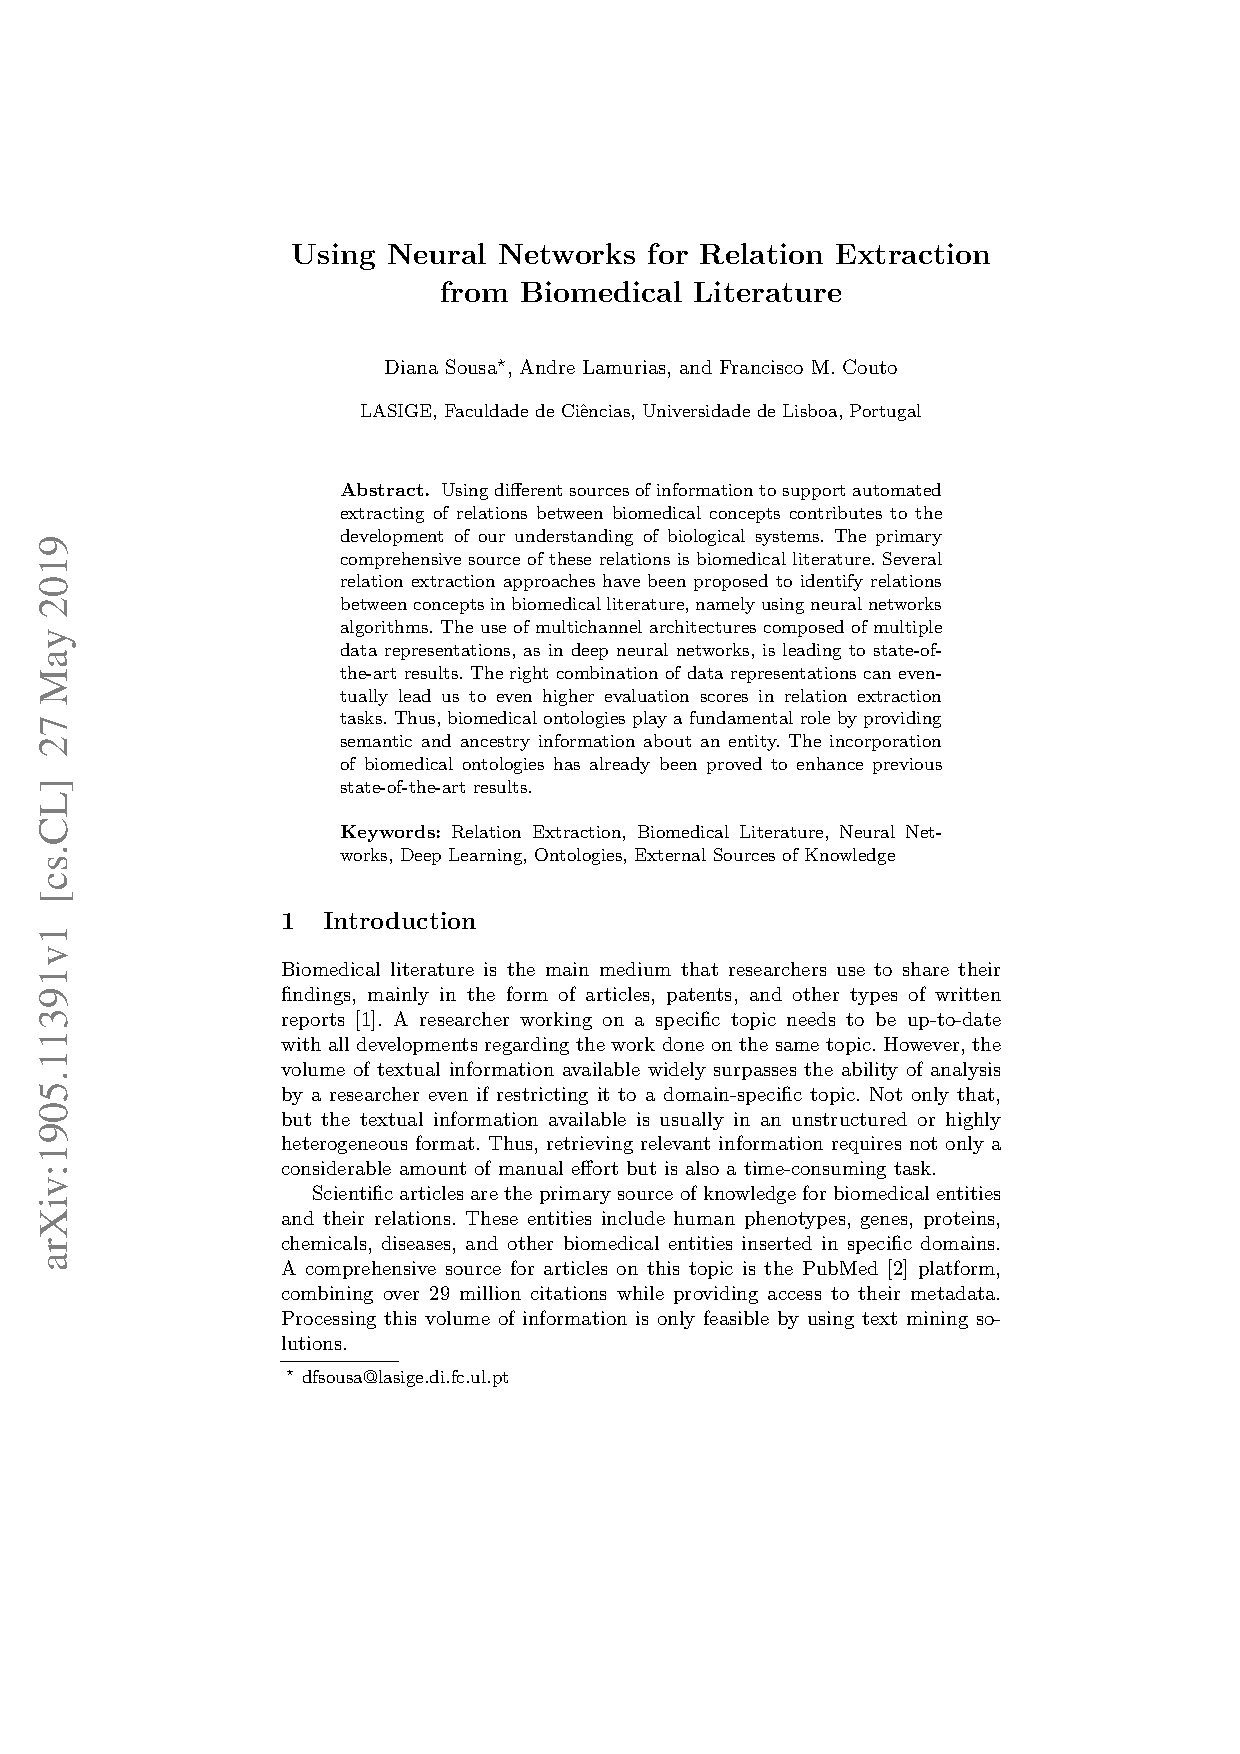
\includepdf[pages=-,scale=1]{articles/1905.11391.pdf}

\hypertarget{AB}{\chapter{BiOnt: Deep Learning using Multiple Biomedical Ontologies for Relation Extraction}}
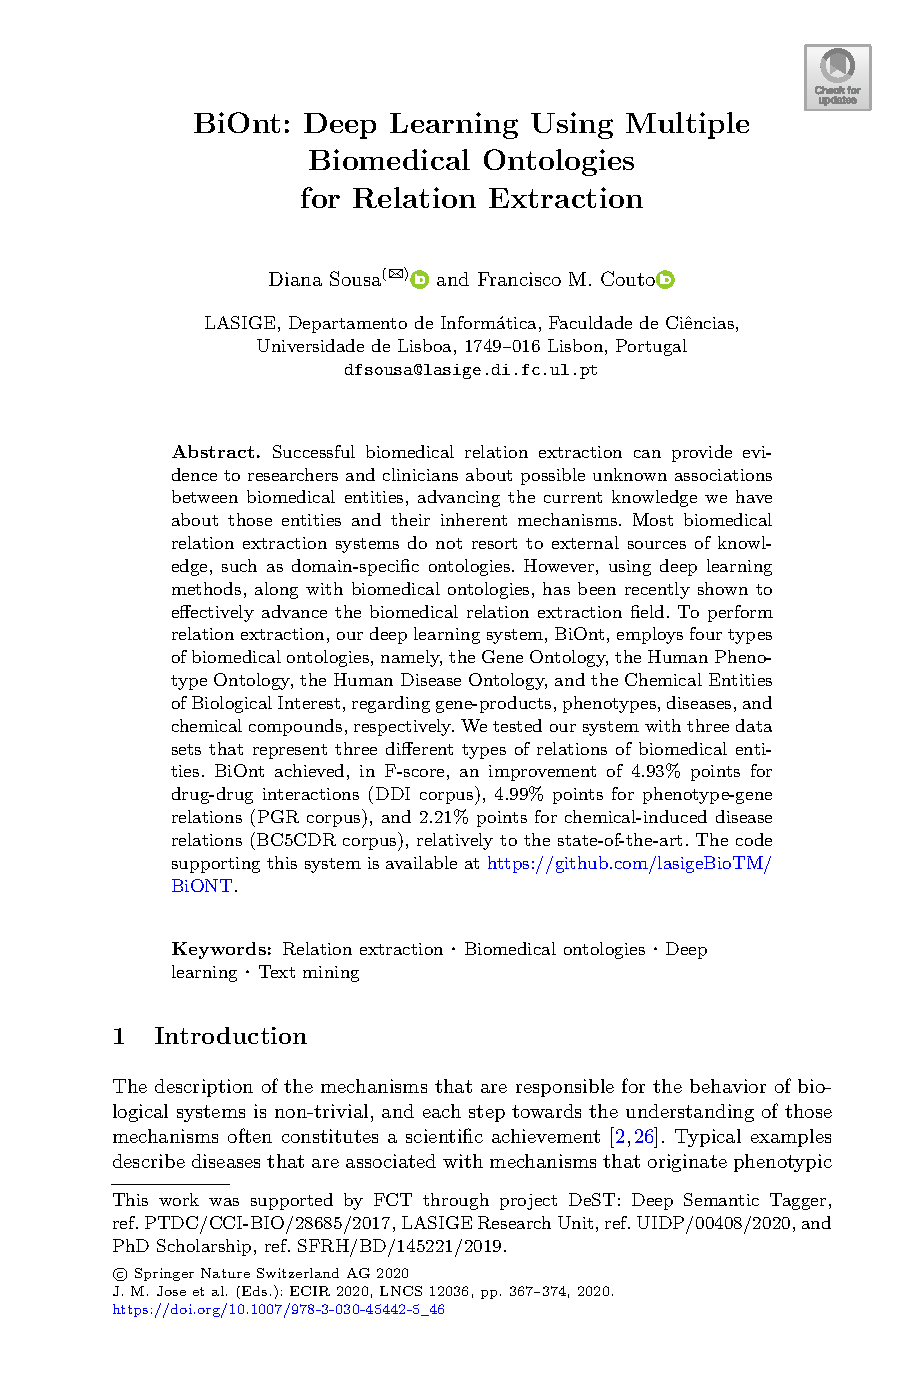
\includepdf[pages=-,scale=0.8]{articles/Sousa-Couto2020_Chapter_BiOntDeepLearningUsingMultiple.pdf}

\hypertarget{AC}{\chapter{Improving Accessibility and Distinction between Negative Results in Biomedical Relation Extraction}}
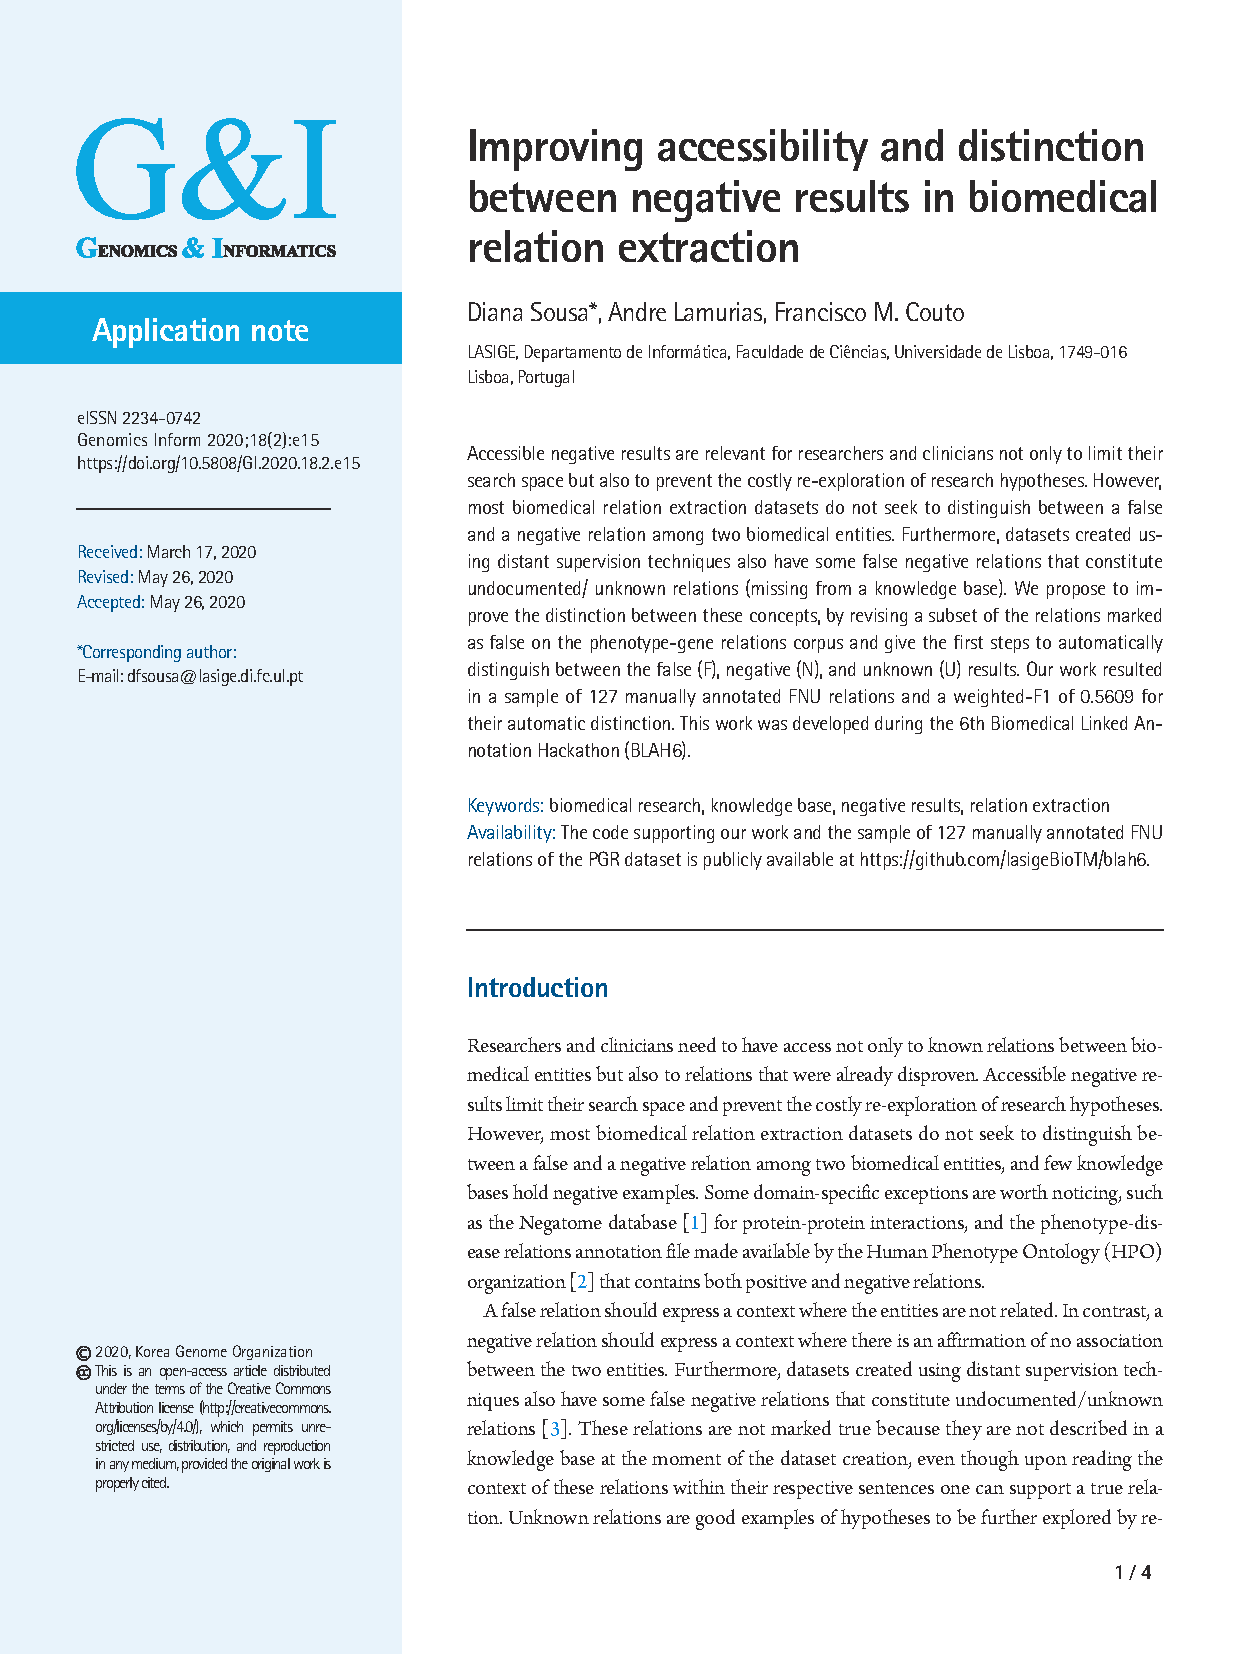
\includepdf[pages=-,scale=0.8]{articles/g_and_i.pdf}

\hypertarget{AD}{\chapter{A Hybrid Approach towards Biomedical Relation Extraction Training Corpora: Combining Distant Supervision with Crowdsourcing}}
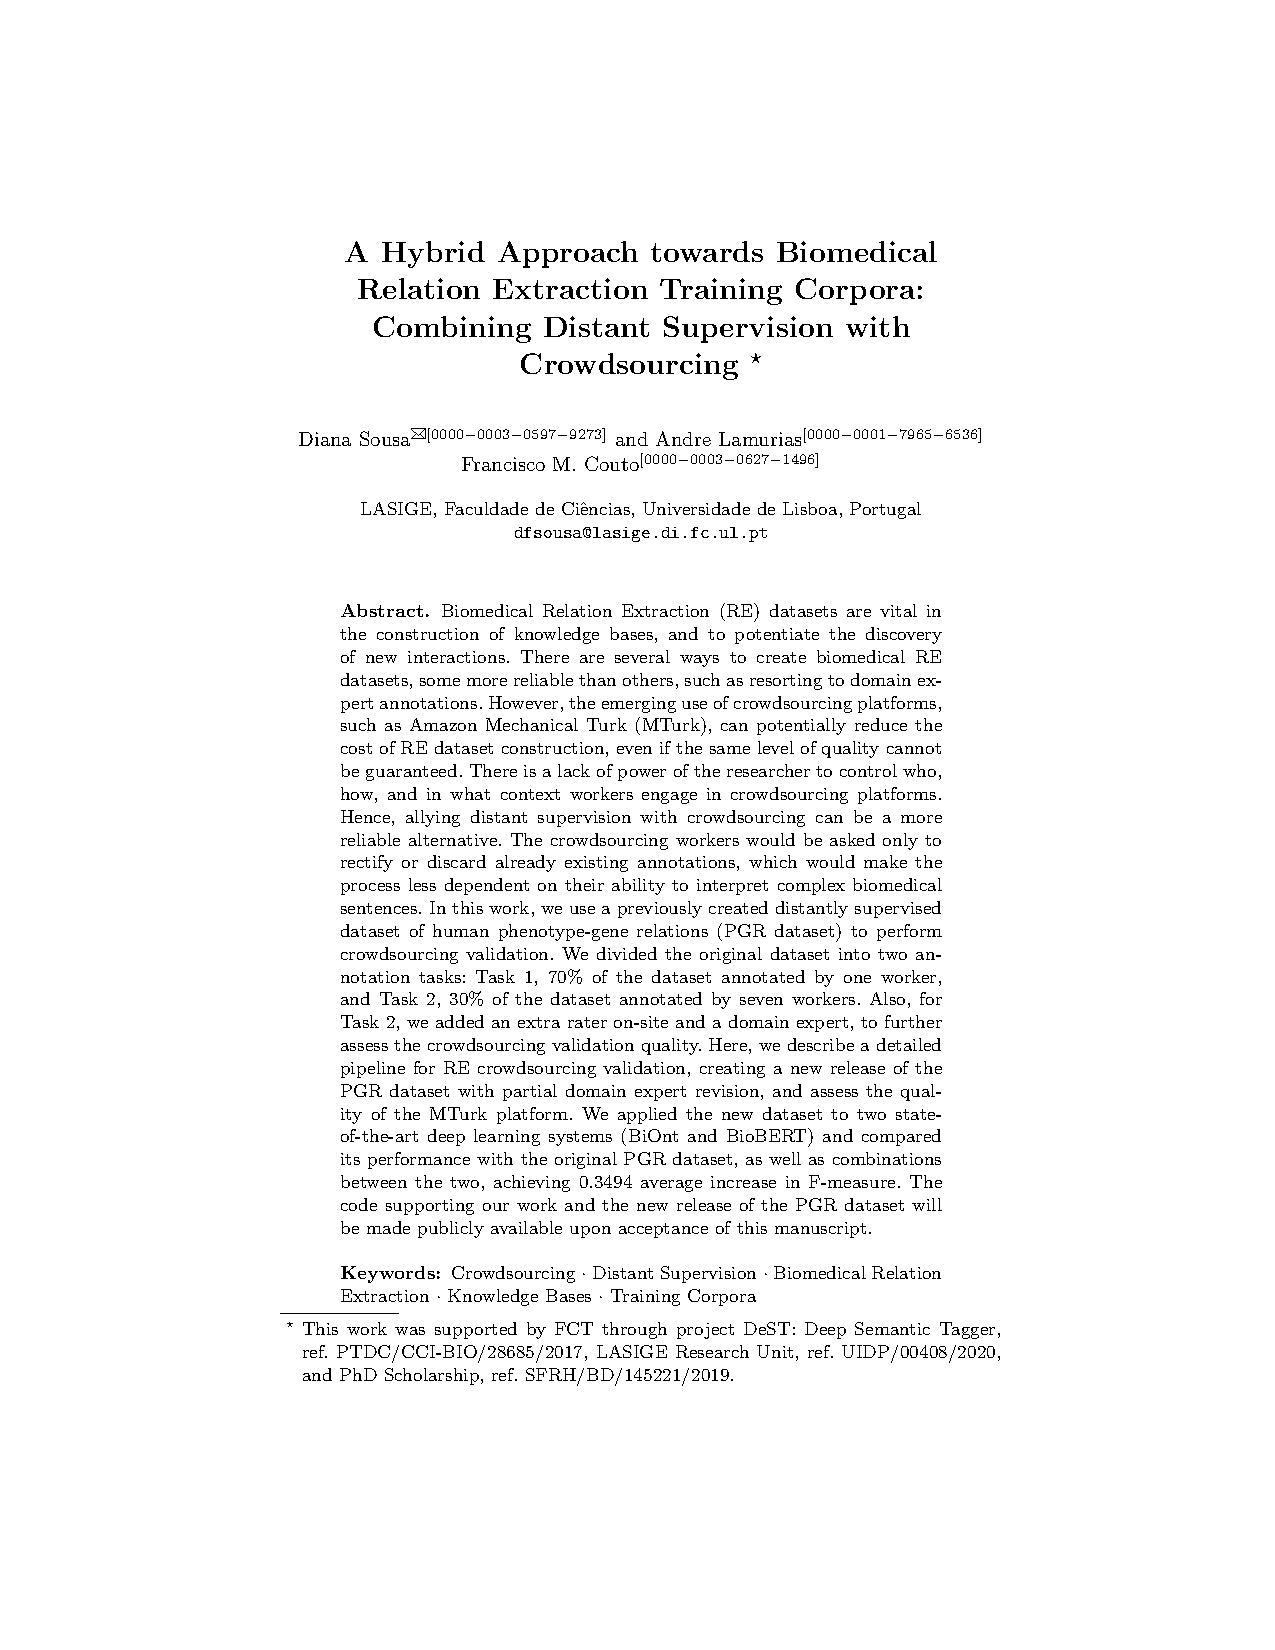
\includepdf[pages=-,scale=1]{articles/DATABASE_preprint.pdf}



\end{document}